%****************************************************************%
%                                                                %
% Modello di tesi di laurea o di dottorato di Lorenzo Pantieri © %
%                                                                %
%         versione: 28 agosto 2012                               %
%                                                                %
%****************************************************************%

% I seguenti commenti speciali impostano:
% 1. utf8 come codifica di input,
% 2. PDFLaTeX come motore di composizione;
% 3. tesi.tex come documento principale;
% 4. il controllo ortografico italiano per l'editor.

% !TEX encoding = UTF-8 Unicode
% !TEX TS-program = pdflatex
% !TEX root = tesi.tex
% !TEX spellcheck = it-IT

\documentclass[
              11pt,%                        % corpo del font principale
              a4paper,%                     % carta A4
%             twoside,openright,%           % fronte-retro
              oneside,openany,%             % solo fronte
              titlepage,%                   % dopo il titolo deve iniziare una nuova pagina
              %fleqn,%                      % position equations at a fixed indent from the left margin rather than centered in the text column (amsmath option)
              headinclude,,footinclude,%    % testatina e piede di pagina
              BCOR5mm,%                     % rilegatura di 5 mm
              numbers=noenddot,%            % niente punto dopo il numero delle sezioni
              cleardoublepage=empty,%       % pagine vuote senza testatina e piede di pagina
              tablecaptionabove,%           % didascalie in cima alle tabelle
              %draft%                         % sostituire con final quando completato
              ]{scrreprt}                   % classe report di KOMA-Script;

\usepackage[T1]{fontenc}                    % codifica dei font:
                                            % NOTA BENE: richiede una distribuzione *completa* di LaTeX (per esempio TeXLive o MiKTeX *complete*)

\usepackage{textcomp}                       % fix warning with missing font shapes
\usepackage{scrhack}                        % fix warnings when using KOMA with listings package
\usepackage{xspace}                         % to get the spacing after macros right

\usepackage[utf8]{inputenc}                 % codifica di input; anche [latin1] va bene
                                            % NOTA BENE! va accordata con le preferenze dell'editor

\usepackage[english,italian]{babel}         % per scrivere in italiano e in inglese;
                                            % l'ultima lingua (l'italiano) risulta predefinita

\usepackage[suftesi]{frontespizio}          % frontespizo
                                            % per includerlo nel documento bisogna:
                                            % 1. compilare una prima volta tesi.tex;
                                            % 2. compilare a parte tesi-frn.tex, generato dalla compilazione precedente;
                                            % 3. compilare ancora tesi.tex che cercherà il file tesi-frn.pdf

\usepackage{indentfirst}                    % rientra il primo capoverso di ogni sezione

\usepackage{graphicx}                       % immagini

\usepackage{listings}                       % codici

\usepackage[font=small]{quoting}            % citazioni

\usepackage{amsmath,amssymb,amsthm,amsfonts}% matematica

\usepackage[italian]{varioref}              % riferimenti completi della pagina

\usepackage{mparhack,fixltx2e,relsize}      % finezze tipografiche

\usepackage[printonlyused,
            smaller,
            withpage]{acronym}              % acronimi

\usepackage{tabularx}                       % tabelle di larghezza prefissata
%\setlength{\extrarowheight}{3pt}           % increase table row height
%\newcommand{\tableheadline}[1]{\multicolumn{1}{c}{\spacedlowsmallcaps{#1}}}
%\newcommand{\myfloatalign}{\centering}     % to be used with each float for alignment
%\usepackage{caption}
%\captionsetup{format=hang,font=small}

\usepackage[babel,
            italian=guillemets]{csquotes}   % rende automatiche alcune scelte stilistiche dipendenti dalla lingua:
                                            % quando viene usato il comando \mkbibquote si otterranno le virgolette orizzontali invece che quelle verticali
\usepackage[style=philosophy-modern,
            hyperref,backref,square,natbib,
            backend=bibtex]{biblatex}       % eccellente pacchetto per la bibliografia;
                                            % philosophy-modern produce uno stile di citazione autore/anno
                                            % aggiungere opzione square dopo backref per parentesti quadrate invece che tonde
                                            % numeric-comp produce riferimenti numerici

\bibliography{bibliografia}                 % database di biblatex

\usepackage{subfig}                         % sottofigure, sottotabelle

\usepackage{lipsum}                         % testo fittizio

\usepackage{eurosym}                        % simbolo dell'euro

% ********************************************************************
% Available options for classicthesis.sty:
% drafting
% parts nochapters linedheaders
% eulerchapternumbers beramono eulermath pdfspacing minionprospacing
% tocaligned dottedtoc manychapters
% listings floatperchapter subfig
% ********************************************************************
\usepackage[eulerchapternumbers,%           % numeri dei capitoli nel font Euler
            subfig,%                        % se si usa il pacchetto subfig
            %minionpro,                    %
            beramono,%                      % Bera Mono come font a spaziatura fissa
            eulermath,%                     % AMS Euler come font per la matematica
            pdfspacing,%                    % migliora il riempimento di riga
            listings,%                      % codici
%           parts,%                         % da decommentare in un documento diviso in parti
            dottedtoc,%                     % allinea a destra i numeri di pagina nell'indice
            floatperchapter                 % numerazione per capitolo dei float (e.g. tabelle, figure, listings)
            ]{classicthesis}                % stile classicthesis


\usepackage{arsclassica}                    % modifica alcuni aspetti di classicthesis

\usepackage{bookmark}                       % segnalibri

\usepackage{etoolbox}

\usepackage{cleveref}

\usepackage{chngcntr}

\usepackage{makeidx}                        % indice analitico

\usepackage{multicol}

%*********************************************************************************
% impostazioni-tesi.tex
% file che contiene le impostazioni della tesi
%*********************************************************************************

%*********************************************************************************
% Comandi personali
%*******************************************************
\newcommand{\myName}{Leonardo Di Donato}% autore
\newcommand{\myTitle}{Continuos Time Bayesian Networks Classifier}% titolo
\newcommand{\myDegree}{Tesi di laurea magistrale}% tipo di tesi
\newcommand{\myUni}{Universit� degli Studi di Milano--Bicocca}% universit�
\newcommand{\myFaculty}{Facolt� di Scienze Matematiche, Fisiche e Naturali}% facolt�
\newcommand{\myDepartment}{Dipartimento di Informatica, Sistemistica e Comunicazione}% dipartimento
\newcommand{\myProf}{Prof.~F.~Antonio Stella}% relatore
\newcommand{\myOtherProf}{Dott.~Daniele Codecasa}% correlatore
\newcommand{\myLocation}{Milano}% dove
\newcommand{\myTime}{Marzo 2013}% quando

%*********************************************************************************
% Impostazioni di amsmath, amssymb, amsthm
%*********************************************************************************
% comandi per gli insiemi numerici (serve il pacchetto amssymb)
\newcommand{\numberset}{\mathbb} 
\newcommand{\N}{\numberset{N}} 
\newcommand{\R}{\numberset{R}} 

% un ambiente per i sistemi
\newenvironment{sistema}%
  {\left\lbrace\begin{array}{@{}l@{}}}%
  {\end{array}\right.}

% definizioni (serve il pacchetto amsthm)
\theoremstyle{definition} 
\newtheorem{definizione}{Definizione}

% teoremi, leggi e decreti (serve il pacchetto amsthm)
\theoremstyle{plain} 
\newtheorem{teorema}{Teorema}
\newtheorem{legge}{Legge}
\newtheorem{decreto}[legge]{Decreto}
\newtheorem{murphy}{Murphy}[section]

% comandi per le lettere greche
\renewcommand{\epsilon}{\varepsilon}
\renewcommand{\theta}{\vartheta}
\renewcommand{\rho}{\varrho}
\renewcommand{\phi}{\varphi}

%*********************************************************************************
% Impostazioni di biblatex
%*********************************************************************************
\defbibheading{bibliography}{%
\cleardoublepage
\manualmark
\phantomsection 
\addcontentsline{toc}{chapter}{\tocEntry{\bibname}}
\chapter*{\bibname\markboth{\spacedlowsmallcaps{\bibname}}
{\spacedlowsmallcaps{\bibname}}}}

%*********************************************************************************
% Impostazioni di listings
%*********************************************************************************
\lstset{language=[LaTeX]Tex,%C++,
    keywordstyle=\color{RoyalBlue},%\bfseries,
    basicstyle=\small\ttfamily,
    %identifierstyle=\color{NavyBlue},
    commentstyle=\color{Green}\ttfamily,
    stringstyle=\rmfamily,
    numbers=none,%left,%
    numberstyle=\scriptsize,%\tiny
    stepnumber=5,
    numbersep=8pt,
    showstringspaces=false,
    breaklines=true,
    frameround=ftff,
    frame=single
}

%*********************************************************************************
% Impostazioni di hyperref
%*********************************************************************************
\hypersetup{%
    hyperfootnotes=false,pdfpagelabels,
    %draft,	% = elimina tutti i link (utile per stampe in bianco e nero)
    colorlinks=true, linktocpage=true, pdfstartpage=1, pdfstartview=FitV,%
    % decommenta la riga seguente per avere link in nero (per esempio per la stampa in bianco e nero)
    %colorlinks=false, linktocpage=false, pdfborder={0 0 0}, pdfstartpage=1, pdfstartview=FitV,% 
    breaklinks=true, pdfpagemode=UseNone, pageanchor=true, pdfpagemode=UseOutlines,%
    plainpages=false, bookmarksnumbered, bookmarksopen=true, bookmarksopenlevel=1,%
    hypertexnames=true, pdfhighlight=/O,%nesting=true,%frenchlinks,%
    urlcolor=webbrown, linkcolor=RoyalBlue, citecolor=webgreen, %pagecolor=RoyalBlue,%
    %urlcolor=Black, linkcolor=Black, citecolor=Black, %pagecolor=Black,%
    pdftitle={\myTitle},%
    pdfauthor={\textcopyright\ \myName, \myUni, \myFaculty},%
    pdfsubject={},%
    pdfkeywords={},%
    pdfcreator={pdfLaTeX},%
    pdfproducer={LaTeX with hyperref and classicthesis}%
}

%*********************************************************************************
% Impostazioni di graphicx
%*********************************************************************************
\graphicspath{{immagini/}} % cartella dove sono riposte le immagini

%*********************************************************************************
% Margini ottimizzati per l'A4
%*********************************************************************************
\areaset[current]{336pt}{750pt}
\setlength{\marginparwidth}{7em}
\setlength{\marginparsep}{2em}%

%*********************************************************************************
% Acronimi
%*********************************************************************************
%\PassOptionsToPackage{printonlyused,smaller}{acronym}
%  \usepackage{acronym} % nice macros for handling all acronyms in the thesis
%\renewcommand*{\acsfont}[1]{\textssc{#1}} % for MinionPro
%\renewcommand{\bflabel}[1]{{#1}\hfill} % fix the list of acronyms

%*********************************************************************************
% Altro
%*********************************************************************************

% ...
\newcommand{\omissis}{[\dots\negthinspace]}

% eccezioni all'algoritmo di sillabazione
\hyphenation{Fortran ma-cro-istru-zio-ne nitro-idrossil-amminico}                   % file con le impostazioni personali

%******************************************************************
% Documento
%******************************************************************
\begin{document}
\pagestyle{scrheadings}
\pagenumbering{roman}
%******************************************************************
% Front matter
%******************************************************************
% !TEX encoding = UTF-8
% !TEX TS-program = pdflatex
% !TEX root = ../tesi.tex
% !TEX spellcheck = it-IT

%*******************************************************
% Frontespizio
%*******************************************************
\begin{frontespizio}
\Preambolo{\usepackage{iwona}} % riga da commentare se non si carica arsclassica

\Universita{Milano--Bicocca}
\Logo{sigillo}
\Facolta{Scienze Matematiche, Fisiche e Naturali}
\Corso{Informatica}
\Annoaccademico{2012--2013}
\Titoletto{Tesi di laurea magistrale}
\Titolo{Continuos Time \\ Bayesian Network Classifiers}
\Sottotitolo{Sottotitolo}
\Candidato[744739]{Leonardo~Di~Donato}
\Relatore{Prof.~F.~Antonio~Stella}
\Correlatore{Dott.~Daniele~Codecasa}
\end{frontespizio}

%*******************************************************
% Frontespizio alternativo
%*******************************************************
%\begin{titlepage}
%\pdfbookmark{Frontespizio}{Frontespizio}
%\changetext{}{}{}{((\paperwidth - \textwidth) / 2) - \oddsidemargin - \hoffset - 1in}{}
%\null\vfill
%\begin{center}
%\large
%\sffamily
%\bigskip

%{\LARGE\myName} \\

%\bigskip

%{\Huge\myTitle \\
%}

%\bigskip
    
%\vspace{9cm}

%\begin{tabular}{cc}
%\parbox{0.3\textwidth}{
\includegraphics[width=2.5cm]{Sigillo}}
%&
%\parbox{0.7\textwidth}{{\Large\myDegree} \\ 

%					{\normalsize
%					Relatore: \myProf \\
%%					Co-relatore: \myOtherProf \\
%					
%					\myUni \\
%					\myFaculty \\
%					\myDepartment \\
%					\myTime}}
%			\end{tabular}
%\end{center}
%\vfill
%\end{titlepage}







% !TEX encoding = UTF-8
% !TEX TS-program = pdflatex
% !TEX root = ../tesi.tex
% !TEX spellcheck = it-IT

%*******************************************************
% Colophon
%*******************************************************
\clearpage
\phantomsection
\thispagestyle{empty}

\hfill

\vfill

%\noindent\myName: \textit{\myTitle,}
%\myDegree,
%\textcopyright\ \MakeTextLowercase{\myTime}.

\lipsum[2]
% !TEX encoding = UTF-8
% !TEX TS-program = pdflatex
% !TEX root = ../tesi.tex
% !TEX spellcheck = it-IT

%*******************************************************
% Dedica
%*******************************************************
\cleardoublepage
\phantomsection
\thispagestyle{empty}
\pdfbookmark{Dedica}{Dedica}

\vspace*{3cm}

\begin{center}
Lorem ipsum dolor sit amet, consectetuer adipiscing elit. \\ \medskip
--- Oscar Wilde    
\end{center}

\medskip

\begin{center}
Dedicato a tutti gli appassionati di \LaTeX.
\end{center}
% !TEX encoding = UTF-8
% !TEX TS-program = pdflatex
% !TEX root = ../tesi.tex
% !TEX spellcheck = it-IT

%*******************************************************
% Indici
%*******************************************************
\cleardoublepage
\pdfbookmark{\contentsname}{tableofcontents}
\setcounter{tocdepth}{2}
\tableofcontents
\markboth{\spacedlowsmallcaps{\contentsname}}{\spacedlowsmallcaps{\contentsname}} 
\clearpage

\begingroup 
    \let\clearpage\relax
    \let\cleardoublepage\relax
    \let\cleardoublepage\relax
    
    %*******************************************************
    % Elenco delle figure
    %*******************************************************    
    \phantomsection
    \pdfbookmark{\listfigurename}{lof}
    \listoffigures

    \vspace*{8ex}

    %*******************************************************
    % Elenco delle tabelle
    %*******************************************************
    \phantomsection
    \pdfbookmark{\listtablename}{lot}
    \listoftables
        
    \vspace*{8ex}
       
\endgroup

\cleardoublepage

% !TEX encoding = UTF-8
% !TEX TS-program = pdflatex
% !TEX root = ../tesi.tex
% !TEX spellcheck = it-IT

%*******************************************************
% Sommario+Abstract
%*******************************************************
\cleardoublepage
\phantomsection
\pdfbookmark{Sommario}{Sommario}
\begingroup
\let\clearpage\relax
\let\cleardoublepage\relax
\let\cleardoublepage\relax

\chapter*{Sommario}

\lipsum[1]

\vfill

\selectlanguage{english}
\pdfbookmark{Abstract}{Abstract}
\chapter*{Abstract}

\lipsum[2]

\selectlanguage{italian}

\endgroup			

\vfill


% !TEX encoding = UTF-8
% !TEX TS-program = pdflatex
% !TEX root = ../tesi.tex
% !TEX spellcheck = it-IT

%*******************************************************
% Ringraziamenti
%*******************************************************
\cleardoublepage
\phantomsection
\pdfbookmark{Ringraziamenti}{ringraziamenti}

\begin{flushright}{\slshape    
	Lorem ipsum dolor sit amet, consectetuer adipiscing elit. \\
	Ut purus elit, vestibulum ut, placerat ac, adipiscing vitae, felis. \\
	Curabitur dictum gravida mauris.} \\ \medskip
    --- Donald Ervin Knuth
\end{flushright}


\bigskip

\begingroup
\let\clearpage\relax
\let\cleardoublepage\relax
\let\cleardoublepage\relax

\chapter*{Ringraziamenti}

\lipsum[1]

\bigskip
 
\noindent\textit{\myLocation, \MakeTextLowercase{\myTime}}
\hfill ~L.

\endgroup
% !TEX encoding = UTF-8
% !TEX TS-program = pdflatex
% !TEX root = ../tesi.tex
% !TEX spellcheck = it-IT

%*******************************************************
% Introduzione
%*******************************************************
\cleardoublepage
\pdfbookmark{Introduzione}{introduzione}
\chapter*{Introduzione}\label{cap:intro}

% \chapter{Introduzione}\label{cap:intro}

\lipsum[1]

Lorem ipsum dolor sit amet, consectetuer adipiscing elit.
% \begin{description}
% \item[{\hyperref[cap:lorem]{Il primo capitolo}}]
% offre una visione d'insieme della storia di \LaTeX{} e ne vengono presentate le idee di fondo.
% \item[{\hyperref[cap:ipsum]{Il secondo capitolo}}]
% spiega le operazioni, veramente semplici, per installare \LaTeX{} sul proprio calcolatore.
% \item[{\hyperref[cap:dolor]{L'appendice A}}] descrive  sinteticamente le principali norme tipografiche della lingua italiana, utili nella composizione di articoli, tesi o libri.
% \end{description}

\begin{description}
\item[{\hyperref[cap:intro]{Il primo capitolo}}]
offre una visione d'insieme della storia di \LaTeX{} e ne vengono presentate le idee di fondo.
\item[{\hyperref[cap:ctbn]{Il secondo capitolo}}]
offre una visione d'insieme della storia di \LaTeX{} e ne vengono presentate le idee di fondo.
\item[{\hyperref[cap:ctbnc]{Il terzo capitolo}}]
spiega le operazioni, veramente semplici, per installare \LaTeX{} sul proprio calcolatore.
\item[{\hyperref[cap:r]{Il quarto capitolo}}]
descrive sinteticamente le principali norme tipografiche della lingua italiana, utili nella composizione di articoli, tesi o libri.
\item[{\hyperref[cap:esperimenti]{Il quinto capitolo}}]
descrive sinteticamente le principali norme tipografiche della lingua italiana, utili nella composizione di articoli, tesi o libri.
\item[{\hyperref[cap:concl]{Il sesto capitolo}}]
descrive sinteticamente le principali norme tipografiche della lingua italiana, utili nella composizione di articoli, tesi o libri.
\end{description}

% \lipsum[2]

\cleardoublepage
%******************************************************************
% Body matter
%******************************************************************
\pagenumbering{arabic}
% !TEX encoding = UTF-8
% !TEX TS-program = pdflatex
% !TEX root = ../tesi.tex
% !TEX spellcheck = it-IT

%%%%%%%%%%%%%%%%%%%%%%%%%%%%%%%%%%%%%%%%%%%%%%%%%%%%%%%%%%%%%%%%%%%%%%%%%%%%%%%%
\chapter{Continuos time \bn{}}
\label{cap:ctbn}
%%%%%%%%%%%%%%%%%%%%%%%%%%%%%%%%%%%%%%%%%%%%%%%%%%%%%%%%%%%%%%%%%%%%%%%%%%%%%%%%
\acresetall
In questo capitolo si introducono i concetti fondamentali relativi alle \ac{CTBN}. Le \acs{CTBN} sono un framework capace di modellare processi stocastici a tempo continuo e con spazio degli stati discreto.

Prima di affrontare tale argomento si presentano alcuni concetti propedeutici a questo lavoro di tesi: le \ac{BN} e i \mprocess{} (\autoref{sec:fondamenti}).
%%%%%%%%%%%%%%%%%%%%%%%%%%%%%%%%%%%%%%%%%%%%%%%%%%%%%%%%%%%%%%%%%%%%%%%%%%%%%%%%
\section{Fondamenti}
\label{sec:fondamenti}
%%%%%%%%%%%%%%%%%%%%%%%%%%%%%%%%%%%%%%%%%%%%%%%%%%%%%%%%%%%%%%%%%%%%%%%%%%%%%%%%
Le \acl{CTBN} utilizzano concetti e idee provenienti da teorie afferenti l'area statistica e del \keyword{machine learning}. Al fine di conferire alla discussione sulle \acs{CTBN} un quadro iniziale completo ed esauriente, si presentano quindi gli aspetti di maggior rilievo di tali argomenti.
\begin{description}
\item[\bn{}] \hfill \\
Le \acl{CTBN} utilizzano una rappresentazione strutturata dello spazio degli stati propria della teoria delle \acl{BN}. Ne ereditano perciò gli aspetti chiave (\eg{} indipendenza \cond*{}) nonché l'insieme delle tecniche algoritmiche per l'apprendimento e l'inferenza.
\item[Processi di Markov]\label{sec:fondamenti-mp}\hfill \\
Le \acl{CTBN} descrivono la dinamica evolutiva di variabili casuali tramite un \mprocess*{} \omog*{} costituito da un insieme di \mprocess{} \cond{}.
\end{description}

\subsection{\bn{}}
\label{sec:bn}
Una \acl{BN} è un modello grafico probabilistico costituito da un \acf{DAG}\footnote{Un grafo aciclico orientato (anche detto grafo aciclico diretto o digrafo aciclico) è un tipo di grafo che non presenta cicli diretti: comunque si scelga un vertice non è possibile tornare ad esso percorrendo gli archi del grafo.}. I nodi di tale grafo rappresentano un insieme di variabili casuali mentre gli archi evidenziano le dipendenze (e le indipendenze) condizionali fra esse~\citep{Korb2011}.
Una \acs{BN} rappresenta la distribuzione di probabilità congiunta del suo insieme di variabili casuali tramite la distribuzione di probabilità \cond*{} di ognuna di essa (si veda l'\autoref{eq:bn-chain-rule}).
Le \acs{BN} sono quindi modelli grafico probabilistici con cui è possibile modellare in modo probabilistico le relazioni causali tra variabili. Esse risultano molto utili nella rappresentazione e analisi di domini caratterizzati da incertezza. Sono infatti usate in svariate applicazioni di supporto alle decisioni, bioinformatica, biologia computazionale, data mining, information retrieval e \keyword{classificazione}.

\subsubsection{Rappresentazione}
Di seguito si fornisce la definizione formale delle \acl{BN} e si introducono i loro aspetti basilari.

\begin{definizione}[\acl{BN}]
\label{defn:bn}
Una \acl{BN} $\conceptsym{B}$ è una coppia $\conceptsym{B}=(\conceptsym{G},\param{$\theta$}_{\conceptsym{G}})$ costituita da:
\begin{itemize}
    \item $\conceptsym{G}=(\set{V}(\conceptsym{G}),\set{A}(\conceptsym{G}))$, un \acl{DAG} dove:
    \begin{itemize}
        \item $\set{V}(\conceptsym{G})=\{\setel{V_1}, \dotsc, \setel{V_n}\}$ è l'insieme dei nodi, ognuno dei quali è associato ad una \acf{CPD}\footnote{Nel caso di variabili causali discrete, le \acs{CPD} sono rappresentabili come delle tabelle che contengono i valori di probabilità di un nodo in funzione di tutte le possibili configurazioni dei nodi genitori (cioè l'insieme dei nodi da cui parte un arco che punta al nodo di interesse). Tali tabelle sono spesso chiamate \acf{CPT}.}
        \item $\set{A}(\conceptsym{G})\subseteq\set{V}(\conceptsym{G})\times\set{V}(\conceptsym{G})$ è l'insieme degli archi fra i nodi $\set{V}(\conceptsym{G})$
    \end{itemize}
    \item $\param{$\theta$}_{\conceptsym{G}}$, insieme delle \acs{CPD} dei nodi che specifica $\set{P}_{\conceptsym{B}}$, la distribuzione di probabilità congiunta delle variabili casuali $\set{X}_{\set{V}(\conceptsym{G})}$ a cui corrispondono i nodi $\set{V}(\conceptsym{G})$.
\end{itemize}
\end{definizione}
\begin{osservazione}\label{oss:bn-markov-assumption}
Ogni nodo di una \acs{BN} è condizionalmente indipendente (si veda \autoref{defn:ic}) dai suoi non--discendenti dati i suoi nodi genitori.
\end{osservazione}

La \acs{CPD} di ogni variabile casuale $\setel{X_i}\in\set{X}_{\set{V}(\conceptsym{G})}$ esprime i suoi valori di probabilità in funzione dei valori assunti da $Pa(\setel{X_i})$, notazione con cui denotiamo l'\emph{insieme dei nodi genitori} per ogni nodo o variabile casuale.

Un arco da un nodo genitore verso un nodo figlio di $\conceptsym{G}$ rappresenta una dipendenza diretta fra le corrispettive variabili casuali~\citep[si veda][sezione 14.1]{Russel2003}. I nodi non direttamente connessi rappresentano variabili casuali condizionalmente indipendenti dagli altri nodi (per quanto riguarda il concetto di \emph{indipendenza \cond*{}} si rimanda alla \autoref{defn:ic}).

Prima di procedere con la discussione si introduce la Chain Rule, proprietà fondamentale delle \acs{BN}.

\begin{teorema}[Chain Rule]
Dato un insieme di variabili casuali e una distribuzione di probabilità congiunta definita su di esse è possibile calcolare qualsiasi elemento di tale distribuzione tramite le distribuzioni di probabilità \cond*{} delle variabili casuali.
\end{teorema}

Perciò, dato un insieme di variabili casuali $\setel{A_1},\dotsc,\setel{A_n}$ è possibile calcolare il valore di tale membro della distribuzione di probabilità congiunta applicando la definizione di probabilità \cond*{}:
\[
\set{P}(\setel{A_1},\dotsc,\setel{A_n})=\set{P}(\setel{A_n}\,\arrowvert\,\setel{A_{n-1}},\dotsc,\setel{A_1})\cdot\set{P}(\setel{A_{n-1}},\dotsc,\setel{A_1})\text{.}
\]
Ripetendo tale processo per ogni termine finale si ottiene:
\begin{equation}
\label{eq:chain-rule}
\set{P}\big(\bigcap_{k=1}^{n}\setel{A_k}\big)=\prod_{k=1}^{n}\set{P}\big(\setel{A_k}\,\arrowvert\,\bigcap_{j=1}^{k-1}\setel{A_j}\big)\text{.}
\end{equation}

Applicando l'\autoref{eq:chain-rule} alle \acl{BN} diciamo che la distribuzione di probabilità congiunta $\set{P}_{\conceptsym{B}}$ si \emph{fattorizza} rispetto al grafo $\conceptsym{G}$ se è possibile scrivere:
\begin{equation}\label{eq:bn-chain-rule}
\set{P}_{\conceptsym{B}}(\setel{X_1}, \dotsc, \setel{X_n})=\prod_{i=1}^{n}\set{P}(\setel{X_i}\,\arrowvert\,Pa(\setel{X_i}))\text{.}
\end{equation}
L'\autoref{eq:bn-chain-rule} esprime quindi la \emph{proprietà di fattorizzazione} della distribuzione congiunta del modello grafico, detta \emph{distribuzione di probabilità globale}, ed è ciò che permette di descriverla efficientemente in funzione delle distribuzioni condizionali dei nodi~\citep[][sezione 14.2]{Russel2003}, dette \emph{distribuzioni di probabilità locali}. Questa proprietà contiene in sè il concetto di \emph{proprietà di Markov} (si veda la \autoref{defn:markov-assumption}), il quale attesta che ogni nodo di una \acl{BN} dipende solo ed esclusivamente dai suoi nodi genitori~\citep[][sezione 2.2.4]{Korb2011}. Si noti inoltre, che le \acl{BN} richiedono (\acs{DAG}, \autoref{defn:bn}) che la loro componente $\conceptsym{G}$ non contenga cicli  affinché possano rispettare tale proprietà~\citep[][sezione 14.1]{Russel2003}.

Poiché, come detto, una \acl{BN} stabilisce che ogni nodo, dati i suoi genitori, è \emph{condizionalmente indipendente} da ogni altro nodo che non sia un suo discendente, di seguito introduciamo tale concetto formalmente.
\begin{definizione}[Indipendenza \cond*{}]\label{defn:ic}
Un evento $\setel{A}$ è \emph{condizionalmente indipendente} da un evento $\setel{B}$, data l'evidenza su un evento $\setel{C}$, qualora la conoscenza di $\setel{B}$ non apporta alcuna variazione alla probabilità di $\setel{A}$ rispetto a quella conseguente alla conoscenza di $\setel{C}$.
Formalmente, ciò significa che:
\[
\set{P}(\setel{A},\setel{B}\,\arrowvert\,\setel{C})=\set{P}(\setel{A}\,\arrowvert\,\setel{B},\setel{C})\cdot\set{P}(\setel{B}\,\arrowvert\,\setel{C})=\set{P}(\setel{A}\,\arrowvert\,\setel{C})\cdot\set{P}(\setel{B}\,\arrowvert\,\setel{C})\text{.}
\]
Da cui segue che:
\[
\setel{A}\perp\setel{B}\,\arrowvert\,\setel{C}\iff\set{P}(\setel{A}\,\arrowvert\,\setel{B},\setel{C})=\set{P}(\setel{A}\,\arrowvert\,\setel{C})\text{.}
\]
\end{definizione}
In termini non formali, supponendo di essere nel caso della definizione, cioè di avere una variabile casuale $\setel{A}$ \emph{condizionalmente indipendente} da $\setel{B}$ dato $\setel{C}$, ciò significa che è possibile ignorare $\setel{B}$ poiché essa non ha alcun riflesso sulla distribuzione \cond*{} di $\setel{A}$ quando sia noto l'evento $\setel{C}$.

Si noti che il concetto appena espresso gioca un ruolo importante per i modelli probabilistici, quali sono le \acl{BN}, semplificando i calcoli richiesti per l'inferenza e l'apprendimento. Le \acl{BN} ereditano questi benefici dell'indipendenza \cond*{} come conseguenza della loro definizione (si veda l'\autoref{oss:bn-markov-assumption}). Infatti, la distribuzione \cond*{} di ogni variabile casuale $\setel{X_i}$ dipende solo ed esclusivamente dal valore dei suoi genitori, $Pa(\setel{X_i})$, mentre ignora completamente i valori dei nodi che non discendono da essa, $Nd(\setel{X_i})$.

Grazie alla \autoref{defn:ic} è possibile esprimere in modo formale il concetto appena espresso per ogni nodo $\setel{X_i}\in\set{X}_{\set{V}(\conceptsym{G})}$:
\[
\set{P}(\setel{X_i}\,\arrowvert\,\setel{E},Pa(\setel{X_i}))=\set{P}(\setel{X_i}\,\arrowvert\,Pa(\setel{X_i})) \quad \forall\:\setel{E}\in Nd(\setel{X_i})\text{,}
\]
dove $Nd(\setel{X_i})$ è l'insieme dei nodi non--discendenti (ed $\setel{E}$ è una variabile casuale o un insieme di variabili casuali ad essi associati).
In base a ciò si dice quindi che le \acl{BN} rispettano l'\emph{assunzione locale di Markov}.

\subsubsection{Apprendimento e Inferenza}\acresetall
In questa sezione si descrivono brevemente e a scopo introduttivo i processi di apprendimento e inferenza sulle \acl{BN}.

Il problema dell'apprendimento per le \acl{BN} si divide principalmente in due casi:
\begin{itemize}
    \item apprendere le \acs{CPD}, nota la struttura
    \item apprendere sia le \acs{CPD}, sia la struttura (incognita).
\end{itemize}
In entrambi i casi è di grande aiuto la rappresentazione efficiente delle \acl{BN} che, tramite la \emph{fattorizzazione} della distribuzione di probabilità congiunta, permette di rappresentarla in modo compatto (tramite l'\autoref{eq:bn-chain-rule}) riducendo notevolmente il numero di parametri da calcolare.

Come detto, per specificare completamente una \acl{BN} è necessario rappresentare completamente la distribuzione di probabilità congiunta delle sue variabili tramite la \acl{CPD} di ognuna di esse. In generale, tali distribuzioni condizionali possono avere una qualsiasi forma anche se, al fine di semplificare i calcoli, è comune utilizzare distribuzioni discrete o Gaussiane per modellarle. Nel caso in cui i dati siano parzialmente osservabili solitamente si procede tramite l'algoritmo di \acf{EM}, il quale alterna il calcolo dei valori attesi delle variabili casuali non osservate condizionalmente ai dati osservati con la massimizzazione della likelihood. Tale approccio generalmente converge ai valori di massima probabilità a posteriori per i parametri~\citep[si veda][]{Dempster1977}.

Per l'\emph{apprendimento dei parametri} esistono comunque una varietà di altri approcci possibili~\citep[si veda][]{Heckerman1996} (\eg{} trattare i parametri come variabili casuali sconosciute addizionali) che tuttavia non sono argomento di questo lavoro di tesi.

Si noti che le \acl{BN} non sono solamente un \emph{modello discriminativo ma anche generativo} poiché possono essere utilizzate per soddisfare query arbitrarie, cioè per effettuare \emph{inferenza probabilistica}: calcolare la distribuzione a posteriori di un insieme di variabili casuali data l'osservazione (evidenza) di altre (sfruttando il \emph{teorema di Bayes}). In letteratura~\citep[si veda][]{Heckerman1996} sono stati esplorati molti metodi di \emph{inferenza esatta}, quali ad esempio l'eliminazione tramite integrazione o somma delle variabili non osservate che non fanno parte della query probabilistica o il metodo clique tree proprogation. Questi metodi, come gli altri presenti in letteratura, dati tutti i possibili alberi di decomposizione del grafo, sono esponenziali rispetto alla larghezza minore rilevata fra essi. Per quanto riguarda invece gli algoritmi di \emph{inferenza approssimata} si citano due tra i più comuni: l'importance sampling~\citep{Shachter1990} e i metodi \acf{MCMC} (\emph{Gibbs sampling}, \emph{Metropolis sampling}, e \emph{Hybrid Monte Carlo sampling}), basati sul campionamento stocastico~\citep[si veda][]{Geman1984,Gilks1996,MacKay1998}.

Nel caso in cui non si disponga della struttura di una \acs{BN} è richiesto l'\emph{apprendimento strutturale}. Gli algoritmi per l'apprendimento strutturale delle \acl{BN} possono essere divisi in due famiglie.
\begin{description}
    \item[Algoritmi basati su vincoli] \hfill \\
    Algoritmi che apprendono la struttura del grafo analizzando le relazioni probabilistiche derivanti dalla proprietà di Markov tramite test di indipendenza condizionale e costruendo un grafo che soddisfi le proprietà di \emph{d-separazione}\footnote{Concetto di separazione direzionale tra insieme di nodi collegato al concetto di \emph{indipendenza condizionale}. Ad esempio, quando un insieme di nodi $\set{E}$ \emph{d-separa} un insieme di nodi $\set{X}=\{\,\setel{A}\,,\,\setel{B}\,\}$ allora $\setel{A}$ e $\setel{B}$ sono condizionalmente indipendenti dato $\set{E}$.} corrispondenti. I modelli risultanti sono spesso interpretati come \emph{modelli causali}~\citep{Pearl1988}.
    \item[Algoritmi basati su punteggio] \hfill \\
    Algoritmi che assegnano un punteggio (tramite una funzione di scoring) a tutte le strutture candidate e utilizzando tecniche di ottimizzazione cercano di raggiungere il punteggio massimo. Gli algoritmi di ricerca greedy (\ie{} \emph{golosi}, \emph{aggressivi} o \emph{avidi} a seconda della traduzione preferita dall'inglese) sono la scelta più comune, tuttavia qualsiasi procedura di ricerca può essere usata.
\end{description}

Gli \emph{algoritmi basati su vincoli} sono basati sull'algoritmo \acf{IC} di~\citet{Verma1991} che fornisce un contesto teorico finalizzato all'apprendimento delle strutture dei modelli causali. L'algoritmo \acs{IC} può essere riassunto nei tre passi successivi.
\begin{itemize}
    \item Apprendimento dello scheletro (\ie{} grafo non diretto) della rete. Poiché la ricerca esaustiva non è, nella maggior parte dei casi, computazionalmente realizzabile, tutti gli algoritmi di apprendimento restringono la ricerca al \emph{Markov blanket}\footnote{\label{note:markov-blanket}Il \emph{Markov blanket} di un nodo $\setel{A}$ è un insieme composto dai nodi genitori di $\setel{A}$, dai suoi nodi figli e da tutti i nodi che condividono un figlio con $\setel{A}$.} di ogni nodo.
    \item Impostare la direzione degli archi che fanno parte di una \emph{v-structure}\footnote{Una \emph{v-structure} è una tripla di nodi $\setel{X}_j\rightarrow\setel{X}_i\leftarrow\setel{X}_k$ incidenti su una connessione convergente.}.
    \item Impostare la direzione degli archi fra i nodi rimanenti affinché il vincolo di aciclicità sia rispettato.
\end{itemize}

Gli \emph{algoritmi basati su punteggio} sono invece delle applicazioni dei vari algoritmi di ricerca euristica (\eg{} \emph{hill climbing}, \emph{tabu search}, \emph{best first search}, \emph{simulated annealing}) che utilizzano una funzione di \emph{scoring}. Solitamente la funzione di \emph{scoring} utilizza la probabilità a posteriori dell'insieme dei dati di apprendimento (\ie{} training set), data la struttura in esame, ed è \emph{score-equivalent}, affinché reti che definiscono la stessa distribuzione di probabilità abbiano lo stesso score~\citep{Chickering2013}. Tuttavia, per quanto questi algoritmi siano utilizzati molto frequentemente, essi sono esponenziali rispetto al numero di nodi della struttura del grafo. Inoltre, qualora si utilizzi una strategia di ricerca locale, è possibile che l'algoritmo restituisca come risultato un minimo locale (per evitare questa situazione si ricorre spesso a metodi di ricerca globale quali il \acs{MCMC}). Si fa notare che è possibile ridurre il tempo necessario richiesto per l'apprendimento strutturale fissando un numero massimo di genitori candidati e cercando esaustivamente in insiemi di tale cardinalità una struttura che massimizzi l'informazione mutua fra variabili~\citep[][]{Heckerman1995}.

\subsection{Processi di Markov}
\label{sec:mps}

Sempre al fine di preparare la discussione delle \acl{CTBN} si prosegue presentando alcuni concetti propedeutici relativi ai \mprocess{}, una categoria di processi stocastici con assenza di memoria~\citep{Loeve1978}.

\begin{definizione}[Proprietà di Markov]
\label{defn:markov-assumption}
Secondo la proprietà di Markov gli stati futuri di un processo stocastico sono indipendenti dagli stati passati, avendo evidenza sullo stato presente di tale processo.

Formalmente, un processo stocastico $\setel{X}$ gode di tale proprietà, se e solo se vale la seguente equazione~\citep{Loeve1978}:
\begin{equation}
\label{eq:markov-assumption}
\set{P}(\setel{X}(t + \Delta t)\,\arrowvert\,\setel{X}(t),\,\setel{X}(s))=\set{P}(\setel{X}(t + \Delta t)\,\arrowvert\,\setel{X}(t))\text{,}
\end{equation}
per ogni $s$, e $t$ tali che $s < t < \infty$.

I modelli che rispettano tale proprietà sono detti modelli che rispettano l'\emph{assunzione di Markov}.
\end{definizione}

Di conseguenza la \acl{CPD} degli stati futuri di un processo stocastico che gode di tale proprietà è indipendente dagli stati passati dato quello attuale.

In altri termini ciò indica che lo stato futuro di una variabile casuale è \emph{condizionalmente indipendente} (si veda la \autoref{defn:ic}) dalla sequenza dei suoi stati passati, avendo evidenza sul suo stato presente.

Dalla proprietà di Markov deriva la definizione dei \mprocess{}.

\begin{definizione}[\upcase\mprocess*{}]
Si definisce~\citep{Loeve1978} come \mprocess*{} un processo stocastico che gode della proprietà di Markov.
\end{definizione}

\begin{definizione}[Catena di Markov]
Un \mprocess*{} che può assumere solo un numero finito di stati è solitamente definito come una \emph{catena di Markov}~\citep[si veda][10]{Norris1998}.
\end{definizione}

Esistono due tipi di processi di Markov: omogenei e non. Si procede quindi fornendone le definizioni.

\begin{definizione}[\upcase\mprocess*{} \omog*{}]
\label{defn:homogeneus-markov-process}
Un \mprocess*{} è detto \emph{\omog*{}} qualora $\set{P}(\setel{X}(t + \Delta t)\,\arrowvert\,\setel{X}(t))$ non dipenda dal tempo $t$. Affinché ciò sia vero, ponenedo $t=0$, deve risultare che:
\begin{equation}
\label{eq:homogeneus-markov-process}
\set{P}(\setel{X}(t + \Delta t)\,\arrowvert\,\setel{X}(t))=\set{P}(\setel{X}(\Delta t)\,\arrowvert\,\setel{X}(0))\text{.}
\end{equation}
\end{definizione}
Data quindi una variabile casuale $\setel{X}$ e l'insieme delle sue istanziazioni $val(\setel{X})=\{\,\vectel{x}_1\,,\,\dotsc\,,\,\vectel{x}_J\,\}$, $\setel{X}(t)$ è un processo di Markov \emph{omogeneo, a tempo continuo e stati finiti} se e solo se la sua dinamica è definibile in termini di:
\begin{itemize}
    \item una distribuzione di probabilità iniziale $\priorsign{\set{X}}$ su $val(\setel{X})$
    \item una \im*{} $\imsign{\setel{X}}$.
\end{itemize}

\begin{definizione}[\upcase\im*{}]
\label{defn:im}
Una \acf{IM}, rappresenta un \emph{modello di transizione Markoviano}:
\[
\imsign{\setel{X}}=
\begin{bmatrix}
    -\param{q}_{\setel{x}_1}    & \param{q}_{\setel{x}_1\setel{x}_2}& \cdots & \param{q}_{\setel{x}_1\setel{x}_k}   \\[0.5em]
    \param{q}_{\setel{x}_2\setel{x}_1}  & -\param{q}_{\setel{x}_2}  & \cdots & \param{q}_{\setel{x}_2\setel{x}_k}   \\[0.5em]
    \vdots      & \vdots    & \ddots & \vdots       \\[0.5em]
    \param{q}_{\setel{x}_k\setel{x}_1}  & \param{q}_{\setel{x}_k\setel{x}_2}& \cdots & -\param{q}_{\setel{x}_k}
\end{bmatrix}\text{.}
\]
Lo scopo di un \im*{} è descrivere il comportamento transiente di $\setel{X}$, un \mprocess*{} \omog*{}.
\end{definizione}

Affinché $\imsign{\setel{X}}$ sia una \acl{IM} valida, ogni sua riga deve sommare a $0$:
\[
\param{q}_{\setel{x}_i}=\sum_{i \neq j}\param{q}_{\setel{x}_i\setel{x}_j}\quad\text{con}\quad \param{q}_{\setel{x}_i}\,,\,\param{q}_{\setel{x}_i\setel{x}_j}>0\text{.}
\]

Data quindi una \im*{} $\imsign{\setel{X}}$ essa descrive il comportamento transiente di $\setel{X}(t)$. Se $\setel{X}(0)=\setel{x}_i$ allora il \mprocess*{} \omog*{} (e indicizzato dal tempo $t$) $\setel{X}(t)$ rimarrà nello stato $\setel{x}_i$ una quantità di tempo \emph{esponenzialmente distribuita} rispetto al parametro $\param{q}_{\setel{x}_i}$. Di conseguenza la \emph{funzione di densità} $f$ e la corrispondente \emph{funzione di ripartizione}\footnote{Nel calcolo delle probabilità la funzione di ripartizione di una variabile casuale $\setel{X}$ a valori reali, anche nota come funzione di distribuzione cumulativa, è la funzione che associa a ciascun valore $\setel{x}$ la probabilità che $\setel{X}$ assuma valori minori o uguali ad $\setel{x}$.} $F$ sono:
\begin{equation}
\label{eq:im-distrib}
\begin{split}
f(t) &= \param{q}_{\setel{x}_i}\,\exp(-\param{q}_{\setel{x}_i}\,t)\,,\quad t>0 \\
F(t) &= 1-\exp(-\param{q}_{\setel{x}_i}\,t)\,,\quad t\geq0\text{.}
\end{split}
\end{equation}

Mentre gli elementi sulla diagonale, $\param{q}_{\setel{x}_i}$, codificano una quantità che può essere interpretata come la \emph{\virgolette{probabilità istantanea}} che $\setel{X}$ abbandoni lo stato $\setel{x}_i$, gli elementi non sulla diagonale, $\param{q}_{\setel{x}_{ij}}$, esprimono l'\emph{intensità di transizione} dallo stato $\setel{x}_i$ allo stato $\setel{x}_j$.

Possiamo quindi calcolare:
\begin{itemize}
    \item il \emph{tempo atteso} di una transizione uscente dallo stato $\setel{x}_i$ \[1/\param{q}_{\setel{x}_i}\]
    \item la \emph{\virgolette{probabilità istantanea}} di transizione dallo stato $\setel{x}_i$ allo stato $\setel{x}_j$ \[\param{$\theta$}_{\setel{x}_i\setel{x}_j}=\param{q}_{\setel{x}_i\setel{x}_j}/\param{q}_{\setel{x}_i}\text{.}\]
\end{itemize}

Quindi una \im*{} induce una distribuzione di probabilità locale fattorizzata in due parti:
\begin{itemize}
    \item $\param{q}_{\setel{x}_i}$, che esprime quando avvengono le transizioni attraverso una \emph{distribuzione di probabilità \keywordsub[distribuzione]{esponenziale}}
    \item $\param{$\theta$}_{\setel{x}_{ij}}$, che esprime la \emph{distribuzione di probabilità \keywordsub[distribuzione]{multinomiale}} tra coppie di stati $i \neq j$.
\end{itemize}
La matrice $\imsign{\setel{X}}$ fa in modo che $\setel{X}$ soddisfi la proprietà di Markov poiché il comportamento futuro di $\setel{X}$ è definito solamente in base al suo stato attuale (vale l'\autoref{eq:homogeneus-markov-process}).
\begin{osservazione}
L'\emph{ordine} di una matrice di intensità corrisponde a $k=|val(\setel{X})|\,$, la cardinalità dell'insieme dei valori assunti da $\setel{X}$.
\end{osservazione}
\begin{osservazione}\label{oss:squared-im}
Nel caso in cui $k=2$, la \im*{} $\imsign{\setel{X}}$ è quindi una matrice $2\times2$. Di conseguenza, poiché ogni riga di $\imsign{\setel{X}}$ somma a $0$ per definizione, le \emph{\virgolette{probabilità istantanee}} di transizione fra gli stati di $\setel{X}$ sono sempre pari a $1$.
\end{osservazione}

\begin{definizione}[\upcase\mprocess*{} \cond*{}]
\label{defn:conditional-markov-process}
Un \mprocess*{} le cui intensità di transizione variano nel tempo non in funzione del tempo ma in funzione dei valori assunti ad ogni determinato istante $t$ da un insieme di altre variabili, che evolvono anch'esse come dei processi di Markov, è detto essere un \mprocess*{} \cond*{} (o \mprocess*{} non \omog*{}).

Assumendo quindi che una variabile casuale $\setel{X}$ evolva come un \mprocess*{} $\setel{X}(t)$ e che la sua dinamica sia condizionata da un insieme di altre variabili casuali $Pa(\setel{X})$, anch'esse dei processi di Markov, possiamo definire per tale variabile casuale una \acf{CIM} $\cimsign{\setel{X}}{Pa(\setel{X})}$.

Se specifichiamo una distribuzione di probabilità iniziale su $\setel{X}$ abbiamo così definito un \mprocess*{} il cui comportamento dipende dalle istanziazioni dei valori di $Pa(\setel{X})$.
\end{definizione}

\begin{definizione}[Matrice di intensità \cond*{}]
\label{defn:cim}
Dato un insieme di processi di Markov $Pa(\setel{X})$, una \im*{} \cond*{} $\cimsign{\setel{X}}{Pa(\setel{X})}$ è costituita da un insieme di \im{} $\cimsign{\setel{X}}{pa_i(\setel{x})}$, una per ogni diversa istanziazione $pa_i(\setel{x})$ di $Pa(\setel{X})$~\citep{Stella2012}:
\[
\cimsign{\setel{X}}{Pa(\setel{X})}=\big\{\,\cimsign{\setel{X}}{pa_1(\setel{x})}\,,\,\cimsign{\setel{X}}{pa_2(\setel{x})}\,,\,\dotsc\,,\,\cimsign{\setel{X}}{pa_n(\setel{x})}\,\big\}\text{.}
\]
Ogni matrice di intensità di $\cimsign{\setel{X}}{Pa(\setel{X})}$ è del seguente tipo:\\
\[
\cimsign{\setel{X}}{pa_i(\setel{x})}=
\begin{bmatrix}
-\param{q}_{\setel{x}_1}^{pa_i(\setel{x})}   & \param{q}_{\setel{x}_1\setel{x}_2}^{pa_i(\setel{x})} & \cdots & \param{q}_{\setel{x}_1\setel{x}_k}^{pa_i(\setel{x})}\\[0.5em]
\param{q}_{\setel{x}_2\setel{x}_1}^{pa_i(\setel{x})} & -\param{q}_{\setel{x}_2}^{pa_i(\setel{x})}   & \cdots & \param{q}_{\setel{x}_2\setel{x}_k}^{pa_i(\setel{x})}\\[0.5em]
\vdots           & \vdots           & \ddots & \vdots\\[0.5em]
\param{q}_{\setel{x}_k\setel{x}_1}^{pa_i(\setel{x})} & \param{q}_{\setel{x}_k\setel{x}_2}^{pa_i(\setel{x})} & \cdots & -\param{q}_{\setel{x}_k}^{pa_i(\setel{x})}
\end{bmatrix}
\text{.}
\]
\end{definizione}
Di seguito si presenta un breve esempio finalizzato alla comprensione pratica delle \cim{} (\acs{CIM}) e del loro scopo.
\begin{esempio}\label{ex:cim}\hfill\\
Date due variabili causali, $\setel{E}(t)$ e $\setel{H}(t)$, delle quali la prima modella l'eventualità che un individuo stia mangiando o meno (se $\setel{e}=2$ allora l'individuo sta mangiando, viceversa se $\setel{e}=1$) mentre la seconda modella l'eventualità che lo stesso individuo abbia fame o meno (se $\setel{h}=2$ allora l'individuo è affamato, viceversa se $\setel{h}=1$) e la \cim*{} $\cimsign{\setel{E}}{\setel{H}}$, che è un insieme composto dalle \im{} $\cimsign{\setel{E}}{h=1}$ e $\cimsign{\setel{E}}{h=2}$, è possibile calcolare la probabilità degli eventi della variabile casuale $\setel{E}$ condizionatamente all'evidenza che si possiede sulla variabile casuale $\setel{H}$.
% \[
% \cimsign{\setel{E}}{h=1}=\begin{bmatrix}-0.01 & 0.01 \\ 10 & -10\end{bmatrix}
% \hspace*{30pt}
% \cimsign{\setel{E}}{h=2}=\begin{bmatrix}-2 & 2 \\ 0.01 & -0.01\end{bmatrix}
% \text{.}
% \]
\[
\cimsign{\setel{E}}{h=1}=\kbordermatrix{
\text{} &   1   &   2\cr
1       &  -.01 & .01\cr
2       & 10    & -10
}
\hspace*{25pt}
\cimsign{\setel{E}}{h=2}=\kbordermatrix{
\text{} &   1   &   2\cr
1       &  -2   &   2\cr
2       &   .01 & -.01
}\text{.}\\
\]
Ipotizzando che l'unità temporale corrisponda a un'ora:
\begin{itemize}
    \item un individuo affamato ($\setel{h}=2$) che non sta mangiando ($\setel{e}=1$) inizierà a mangiare in 30 minuti poiché \[\frac{1}{\param{q}_{\setel{e}=1\,\arrowvert\,\setel{h}=2}}=\frac{1}{2}\:\text{,}\]
    \item un individuo non affamato ($\setel{h}=1$) che sta mangiando ($\setel{e}=2$) smetterà di mangiare ($\setel{e}=1$) entro 6 minuti poiché \[\frac{1}{\param{q}_{\setel{e}=2\,\arrowvert\,\setel{h}=1}}=\frac{1}{10}\:\text{;}\] si osservi che la\emph{\virgolette{probabilità istantanea}} di transizione da $\setel{e}=2$ a $\setel{e}=1$, come già evidenziato dall'\autoref{oss:squared-im}, è \[\param{$\theta$}_{\setel{e}=2,\setel{e}=1\,\arrowvert\,\setel{h}=1}=\frac{\param{q}_{\setel{e}=2,\setel{e}=1\,\arrowvert\,\setel{h}=1}}{\param{q}_{\setel{e}=2\,\arrowvert\,\setel{h}=1}}=\frac{10}{10}=1\text{.}\]
\end{itemize}
\end{esempio}

%%%%%%%%%%%%%%%%%%%%%%%%%%%%%%%%%%%%%%%%%%%%%%%%%%%%%%%%%%%%%%%%%%%%%%%%%%%%%%%%
\section{Definizioni preliminari}
\label{sec:Definizioni preliminari}
%%%%%%%%%%%%%%%%%%%%%%%%%%%%%%%%%%%%%%%%%%%%%%%%%%%%%%%%%%%%%%%%%%%%%%%%%%%%%%%%
Nelle precedenti sezioni sono stati illustrati i concetti che si pongono a fondamento delle \acl{CTBN}:
\begin{itemize}
    \item le \acl{BN}: utili a comprendere la rappresentazione strutturata dello spazio degli stati delle \acs{CTBN}, l'utilizzo della nozione di indipendenza \cond*{} e le conseguenti tecniche di apprendimento e inferenza
    \item i \mprocess{}, \omog{} e non, al fine di introdurre le modalità di rappresentazione (qualitativa e quantitativa) delle \acs{CTBN}.
\end{itemize}

Prima di presentare le \acl{CTBN} come una collezione di \ctmp{} non \omog{} e con spazio degli stati discreto~\citep{Nodelman2007}, si forniscono alcune definizioni utili per il prosieguo della discussione.

\begin{definizione}[\acl{PV}]\label{defn:pv}
    Una \pv{} $\set{X}$, anche detta \ACF{PV}~\citep{Nodelman2007}, è un insieme di \ctmp{} $\setel{X}(t)$.
\end{definizione}

\begin{definizione}[Traiettoria]\label{defn:traiettoria}
    Istanziazione di un insieme di valori per $\setel{X}(t)$ al variare di $t$.
\end{definizione}

\begin{definizione}[$J$-time-segment]\label{defn:j-time-segment}
Partizionamento di un intervallo temporale $[\,0,\,T)$ in $J$ intervalli chiusi a sinistra:
\[
[\,0,\,t_1)\:;\:[\,t_1,\,t_2)\:;\:\dotsc\:;\:[\,t_{J-1},\,T)\text{.}
\]
\end{definizione}
\begin{notabene}
\`E possibile riferirsi a tale concetto anche tramite l'espressione \emph{\virgolette{insieme dei \keywordsub[definizione]{segmenti temporali}}}.
\end{notabene}
\begin{definizione}[$J$-evidence-stream]\label{defn:j-evidence-stream}
Dato un insieme di segmenti temporali composto da $J$ intervalli e una \pv{} $\set{X}$ composta da $N$ variabili casuali, un \emph{$J$-evidence-stream} è l'insieme delle istanziazioni comuni $\set{X}=\set{x}$ associate ad ogni intervallo temporale per ogni sottoinsieme delle variabili casuali~\citep{Stella2012}. \`E denotato con $(\set{X}^1=\set{x}^1\,,\,\set{X}^2=\set{x}^2\,,\,\dotsc\,,\,\set{X}^J=\set{x}^J)$, o più concisamente $\evidencestream{J}$.
\end{definizione}
\begin{notabene}
\`E possibile riferirsi a tale concetto anche tramite l'espressione \emph{\virgolette{flusso di evidenze}}.
\end{notabene}
\begin{notabene}
Un flusso di evidenze $\evidencestream{J}$. è detto essere \emph{completamente osservato} se lo stato di tutte le variabili $\setel{X_n}\in\set{X}$ è conosciuto in tutto l'intervallo $[\,0,\,T)$. Viceversa, un flusso di evidenze è detto \emph{parzialmente osservato}.
\end{notabene}

%%%%%%%%%%%%%%%%%%%%%%%%%%%%%%%%%%%%%%%%%%%%%%%%%%%%%%%%%%%%%%%%%%%%%%%%%%%%%%%%
\section{Rappresentazione}
\label{sec:ctbn-rappresentazione}
%%%%%%%%%%%%%%%%%%%%%%%%%%%%%%%%%%%%%%%%%%%%%%%%%%%%%%%%%%%%%%%%%%%%%%%%%%%%%%%%
Una \acl{CTBN} è un modello grafico in cui ogni nodo rappresenta una variabile casuale i cui stati evolvono in modo continuo bel tempo. Le dinamiche evolutive degli stati dei nodi sono governate e dipendono dal valore che gli stati dei nodi padre\footnote{Con il termine \virgolette{nodo padre}, o \emph{parent node}, si intende un nodo il cui stato condiziona quello di un altro nodo del modello grafico.} assumono~\citep{Stella2012}. Quindi ogni nodo è un \mprocess*{} \cond*{} (si veda la \autoref{defn:conditional-markov-process}) a tempo continuo e spazio degli stati discreto.

Una \acs{CTBN} è composta principalmente da due componenti:
\begin{itemize}
    \item una distribuzione di probabilità iniziale
    \item le dinamiche che regolano l'evoluzione nel tempo continuo della distribuzione di probabilità
\end{itemize}
Più formalmente si definisce:
\begin{definizione}[\acl{CTBN}]
\label{defn:ctbn}
Data una \pv{} $\set{X}$, insieme di processi di Markov $\setel{X_1}\,,\,\setel{X_2}\,,\,\dotsc\,,\,\setel{X_N}$ a tempo continuo e con spazio degli stati finito $val(\setel{X_n})=\{\,\vectel{\setel{x}_1}\,,\,\dotsc\,,\,\vectel{\setel{x}_J}\,\}$ (dove $n=1\,,\,\dotsc\,,\,N$), una \acs{CTBN} $\conceptsym{N}$ su $\set{X}$ consiste di:
\begin{itemize}
    \item una distribuzione di probabilità iniziale $\priorsign{\set{X}}$ specificata come una \bn{} $\conceptsym{B}$ su $\set{X}$
    \item un modello di transizione a tempo continuo, specificato da:
    \begin{itemize}
        \item un grafo $\conceptsym{G}$, orientato e non necessariamente aciclico, composto dai nodi $\setel{X_1}\,,\,\setel{X_2}\,,\,\dotsc\,,\,\setel{X_N}$, ognuno dei quali possiede un insieme di genitori denotato da $Pa(\setel{X_n})$
        \item una \im*{} \cond*{} $\cimsign{\setel{X_n}}{Pa(\setel{X_n})}$ per ogni nodo $\setel{X_n} \in \set{X}$.
    \end{itemize}
\end{itemize}
\end{definizione}

Per ogni variabile causale $\setel{X_n} \in \set{X}$ di $\conceptsym{N}$ si ha quindi un insieme di modelli di probabilità locali: $\cimsign{\setel{X_n}}{Pa(\setel{X_n})}$, la \acs{CIM} di $\setel{X_n}$, è infatti un insieme di modelli di transizione Markoviani la cui cardinalità è pari a quella dell'insieme delle diverse istanziazioni di $Pa(\setel{X_n})$.

Si riscontra, quindi, quanto già affermato in precedenza (si veda \ref{sec:fondamenti-mp}), cioè che una \acs{CTBN} esprime la sua dinamica evolutiva globale tramite un unico \mprocess*{} \omog*{}, costituito da un insieme di \mprocess{} \cond{} (un insieme di \acs{CIM} e relative distribuzioni di probabilità iniziali).

Si noti che, diversamente dalle \acl{BN}, nelle \acl{CTBN} gli archi fra i nodi rappresentano le dipendenze nel tempo. Per tale motivo è possibile che la componente $\conceptsym{G}$ del modello di transizione continuo contenga dei cicli. Tra l'altro, come vedremo nel prosieguo, la mancanza di tale vincolo di aciclicità porta a notevoli vantaggi computazionali relativamente all'apprendimento della struttura di una \acs{CTBN} dai dati.

%%%%%%%%%%%%%%%%%%%%%%%%%%%%%%%%%%%%%%%%%%%%%%%%%%%%%%%%%%%%%%%%%%%%%%%%%%%%%%%%
\section{Apprendimento}
\label{sec:ctbn-apprendimento}
%%%%%%%%%%%%%%%%%%%%%%%%%%%%%%%%%%%%%%%%%%%%%%%%%%%%%%%%%%%%%%%%%%%%%%%%%%%%%%%%
In questa sezione si argomenta sulla probabilità di un \emph{insieme di dati completo} rispetto a una \acl{CTBN}. A tal fine si mostra come una \acs{CTBN}, essendo un modello esponenziale, possa essere decomposta in un aggregato di modelli di probabilità locali relativi alle singole variabili casuali e espressa in termini di \emph{\stats{}} aggregate.

Si affronta infine il processo di apprendimento dei parametri delle \acl{CTBN} da \emph{dati completi}. I processi di apprendimento relativi a dati non completi sono tralasciati poiché non facenti parte degli argomenti di questo lavoro di tesi.

\begin{definizione}[Insieme di dati completo]
\label{defn:dataset-completo}
Dato un insieme di variabili casuali, un insieme di dati $\conceptsym{D}=\{\,\delta_1\,,\,\dotsc\,,\,\delta_h\,\}$ si dice \emph{completo} se ogni $\delta_i$ (con $i=1\,,\,\dotsc\,,\,h$) è un insieme di traiettorie completamente osservate delle variabili casuali (\ie{} l'istanziazione di tutte le variabili casuali è osservabile per ogni istante temporale di ogni traiettoria).
\end{definizione}

\subsection{Statistiche sufficienti}
\label{sec:ctbn-sufficient-stats}
Le \emph{\stats{}} per un singolo \mprocess*{} \omog*{} $\setel{X}(t)$ riassumono la sua dinamica evolutiva con:
\begin{itemize}
    \item $\tstat{x}$: la quantità di tempo trascorsa nello stato $\setel{x}$
    \item $\mstat[x]{\setel{x}^\prime}$: il numero di transizioni dallo stato $\setel{x}$ allo stato $\setel{x}^\prime$.
\end{itemize}

Il numero totale di transizioni uscenti da uno stato $\setel{x}$ è:
\[
\mstat{x}=\sum_{\setel{x}^\prime}\mstat[x]{\setel{x}^\prime}\text{.}
\]
Nel caso di un \mprocess*{} \cond*{} è invece necessario considerare anche l'istanziazione dell'insieme $Pa(\setel{X})$ dei nodi genitori:
\begin{itemize}
    \item $\tstat{x\,\arrowvert\,pa_i(\setel{x})}$: la quantità di tempo trascorsa nello stato $\setel{x}$ quando $Pa(\setel{X})=pa_i(\setel{x})$
    \item $\mstat[x]{\setel{x}^\prime\,\arrowvert\,pa_i(\setel{x})}$: il numero di transizioni dallo stato $\setel{x}$ allo stato $\setel{x}^\prime$ quando $Pa(\setel{X})=pa_i(\setel{x})$.
\end{itemize}
Chiaramente, il numero totale di transizioni si calcola come sopra.

\subsection{Likelihood}
\label{sec:ctbn-likelihood}
Al fine di presentare il calcolo della likelihood\footnote{\label{note:likelihood}La likelihood di un insieme di valori per i parametri, dato un insieme di dati, è uguale alla probabilità dei dati, dati tali valori per i parametri.} di una \acs{CTBN} rispetto a un dataset completo $\conceptsym{D}$ è bene procedere per gradi e iniziare presentando dapprima la likelihood di una singola transizione di un singolo \mprocess*{} \omog*{} $\setel{X}(t)$.

\subsubsection{Likelihood di una singola transizione}
\label{sec:ctbn-likelihood-single-trans-single-hmp}
Data una tripla $d=\langle \,\setel{x}_{d}\,,\,t_d\,,\,\setel{x}_{d^{\prime}}\,\rangle\in\conceptsym{D}$, la quale esprime una transizione di $\setel{X}(t)$ da $\setel{x}_d$ a $\setel{x}_{d^{\prime}}$ dopo che esso ha trascorso $t_d$ tempo in $\setel{x}_d$, è possibile scrivere la likelihood di questa singola transizione $d$ in funzione dei parametri (\ref{sec:ctbn-params}):
\begin{equation}
\label{eq:ctbn-trans-hmm-likelihood}
\begin{split}
L_{\setel{X}}(\param{q}\,,\,\param{$\theta$}:d) &= L_{\setel{X}}(\param{q}:d)\,L_{\setel{X}}(\param{$\theta$}:d) \\
&= \param{q}_{\setel{x}_d}\,\exp(-\param{q}_{\setel{x}_d}\,t_d)\,(\param{$\theta$}_{\setel{x}_{d}\setel{x}_{d^{\prime}}})\text{.}
% &= \param{q}_{\setel{x}_d}\,\exp(-\param{q}_{\setel{x}_d}\,t_d)\,\Big(\frac{\param{q}_{\setel{x}_{d}\setel{x}_{d^{\prime}}}}{\param{q}_{\setel{x}_d}}\Big) \\
% &= \exp(-\param{q}_{\setel{x}_d}\,t_d)\,\param{q}_{\setel{x}_{d}\setel{x}_{d^{\prime}}}
\end{split}
\end{equation}
Si noti che l'\autoref{eq:ctbn-trans-hmm-likelihood} è ricavata moltiplicando la \emph{funzione di distribuzione di probabilità} di $\setel{X}(t)$ (\autoref{eq:im-distrib}) per la \emph{\virgolette{probabilità istantanea}} di transizione (si veda la \autoref{defn:im}).

\subsubsection{Likelihood di un dataset completo}
\label{sec:ctbn-likelihood-dataset}
Poiché tutte le transizioni sono osservabili, la \emph{likelihood} del dataset $\conceptsym{D}$ può essere decomposta come un prodotto delle likelihood individuali di ogni singola transizione $d$~\citep[si veda][3]{Nodelman2002}. Per tale motivo $\conceptsym{D}$ è sintentizzabile aggregando le \emph{\stats{}} relative a ogni \mprocess*{} \cond*{} di una \acs{CTBN}.

Quindi la likelihood di un dataset completo $\conceptsym{D}$ rispetto a un singolo \mprocess*{} \omog*{} $\setel{X}(t)$ è:
\begin{equation}
\label{eq:ctbn-data-hmp-likelihood}
\begin{split}
L_{\setel{X}}(\param{q}\,,\,\param{$\theta$}:\conceptsym{D})&=\bigg[\prod_{d\in\conceptsym{D}}L_{\setel{X}}(\param{q}:d)\bigg]\bigg[\prod_{d\in\conceptsym{D}}L_{\setel{X}}(\param{$\theta$}:d)\bigg]\\[5pt]
&=\Big[\prod_{\setel{x}}\param{q}_{\setel{x}}^{\mstat{x}}\exp(-\param{q}_{\setel{x}}\tstat{x})\Big]\Big[\prod_{x}\prod_{x\neq x^{\prime}}\param{$\theta$}_{\setel{x}\setel{x}^{\prime}}^{\mstat[x]{\setel{x}^\prime}}\Big]\text{.}
\end{split}
\end{equation}
Si supponga ora di traslare questo concetto a una \acl{CTBN} $\conceptsym{N}$ con $N$ nodi: per ogni nodo $\setel{X_i}$, con $i=1\,,\,\dotsc\,N$ è necessario considerare tutte le transizioni contestualmente all'istanziazione dell'insieme $Pa(\setel{X_i})$ dei suoi nodi genitori. Poiché, nel caso di \emph{dati completi}, si conosce sempre l'istanziazione di $Pa(\setel{X_i})$, allora, per ogni istante di tempo $t$, si conosce quale \im*{} $\cimsign{\setel{X_i}}{pa_i(\setel{x})}\,$, con $pa_i(\setel{x})\in Pa(\setel{X_i})\,$, governi la dinamica di $\setel{X_i}$.

Perciò la probabilità dei dati $\conceptsym{D}$ rispetto a $\conceptsym{N}$ è il prodotto delle likelihood di ogni variabile $\setel{X_i}$:
\begin{equation}
\begin{split}
L_{\conceptsym{N}}(\param{q}\,,\,\param{$\theta$}\,:\conceptsym{D})&=\prod_{\setel{X}_i\in\set{X}}L_{\setel{X}_i}(\param{q}_{\setel{X}_i\,\arrowvert\,Pa(\setel{X}_i)}\,,\,\param{$\theta$}_{\setel{X}_i\,\arrowvert\,Pa(\setel{X}_i)}:\conceptsym{D}) \\
&=\prod_{\setel{X}_i\in\set{X}}L_{\setel{X}_i}(\param{q}_{\setel{X}_i\,\arrowvert\,Pa(\setel{X}_i)}:\conceptsym{D})\,L_{\setel{X}_i}(\param{$\theta$}_{\setel{X}_i\,\arrowvert\,Pa(\setel{X}_i)}:\conceptsym{D})\text{.}
\end{split}
\end{equation}
Il termine $L_{\setel{X}}(\param{$\theta$}_{\,\setel{X}\,\arrowvert\,Pa(\setel{X})}:\conceptsym{D})$ esprime la likelihood delle transizioni tra stati. Si osservi, inoltre, come il tempo che intercorre fra le transizioni sia trascurato poiché esse dipendono esclusivamente dal valore di nodi genitori~\citep[si veda][3]{Nodelman2002}. Quindi, usando le \emph{\stats{}} si può scrivere:
\[
L_{\setel{X}}(\param{$\theta$}_{\,\setel{X}\,\arrowvert\,Pa(\setel{X})}:\conceptsym{D})=\prod_{pa_i(\setel{x})} \prod_{x} \prod_{x\neq x^{\prime}}\param{$\theta$}_{xx^{\prime}\,\arrowvert\,pa_i(\setel{x})}^{\mstat[x]{\setel{x}^{\prime}\,\arrowvert\,pa_i(\setel{x})}}\text{.}
\]

Per quanto riguarda il calcolo di $L_{\setel{X}}(\param{q}_{\,\setel{X}\,\arrowvert\,Pa(\setel{X})}:\conceptsym{D})$ va considerato il caso in cui il tempo trascorso da $X$ in uno determinato stato $\setel{x}$ termini non a causa di una sua transizione bensì a causa di una transizione di uno o più nodi appartenenti all'insieme dei suoi nodi genitori (\ie{} una nuova istanziazione per l'insieme dei genitori $Pa(\setel{X})$). \`E quindi necessario considerare la probabilità che il nodo $X$ rimanga in $x$ una quantità di tempo \emph{almeno pari} a $t$ mentre i suoi nodi genitori $Pa(\setel{X})$ non effettuano alcuna transizione di stato~\citep[si veda][3]{Nodelman2002}. Tale quantità si ricava dalla funzione di distribuzione cumulativa di una distribuzione \keywordsub[distribuzione]{esponenziale} (\autoref{eq:im-distrib}):
\[
1-F(t)=\exp(-\param{q}_{\setel{x}\,\arrowvert\,pa_i(\setel{x})} t)\text{.}
\]
Perciò la likelihood delle quantità di tempo trascorse in ogni stato è:
\small
\[
L_{\setel{X}}(\param{q}_{\,\setel{X}\,\arrowvert\,Pa(\setel{X})}:\conceptsym{D})=\prod_{pa_i(\setel{x})}\prod_{x}\param{q}_{x\,\arrowvert\,pa_i(\setel{x})}^{\mstat{x\,\arrowvert\,pa_i(\setel{x})}}\exp(-\param{q}_{\setel{x}\,\arrowvert\,pa_i(\setel{x})}\,\tstat{\setel{x}\,\arrowvert\,pa_i(\setel{x})})\text{\normalsize .}
\]
\normalsize
La likelihood di $\conceptsym{N}$ è quindi:
% \begin{equation}
% \label{eq:ctbn-likelihood}
% \resizebox{.92\hsize}{!}{$L_{\conceptsym{N}}(\param{q}\,,\,\param{$\theta$}\,:\conceptsym{D})=\prod_{pa_i(\setel{x})}\prod_{x}\Big(\param{q}_{x\,\arrowvert\,pa_i(\setel{x})}^{\mstat{x\,\arrowvert\,pa_i(\setel{x})}}\exp(-\param{q}_{x\,\arrowvert\,pa_i(\setel{x})}\,\tstat{x\,\arrowvert\,pa_i(\setel{x})})\,\prod_{x\neq x^{\prime}}\param{$\theta$}_{xx^{\prime}\,\arrowvert\,pa_i(\setel{x})}^{\mstat[x]{x^{\prime}\,\arrowvert\,pa_i(\setel{x})}}\Big)$}\text{.}
% \end{equation}
{
\footnotesize
\begin{equation}\label{eq:ctbn-likelihood}
\begin{split}
L_{\conceptsym{N}}(\param{q}\,,\,\param{$\theta$}\,:\conceptsym{D}) &= \prod_{pa_i(\setel{x})}\prod_{\setel{x}}\bigg[\param{q}_{\setel{x}\,\arrowvert\,pa_i(\setel{x})}^{\mstat{x\,\arrowvert\,pa_i(\setel{x})}}\exp(-\param{q}_{\setel{x}\,\arrowvert\,pa_i(\setel{x})}\,\tstat{x\,\arrowvert\,pa_i(\setel{x})})\:\cdot \\
& \quad \cdot \prod_{\setel{x}\neq \setel{x}^{\prime}}\param{$\theta$}_{\setel{x}\setel{x}^{\prime}\,\arrowvert\,pa_i(\setel{x})}^{\mstat[x]{\setel{x}^{\prime}\,\arrowvert\,pa_i(\setel{x})}}\bigg]\text{\normalsize .}
\end{split}
\end{equation}
}
\normalsize
Mentre, scrivendola come \emph{log-likelihood}, si ottiene:
{
\footnotesize
\begin{equation}\label{eq:ctbn-log-likelihood}
\begin{split}
\ell_{\conceptsym{N}}(\param{q}\,,\,\param{$\theta$}\,:\conceptsym{D}) &= \sum_{pa_i(\setel{x})}\sum_{\setel{x}}\bigg[\mstat{x\,\arrowvert\,pa_i(\setel{x})}\ln(\param{q}_{x\,\arrowvert\,pa_i(\setel{x})})- \param{q}_{\setel{x}\,\arrowvert\,pa_i(\setel{x})}\tstat{\setel{x}\,\arrowvert\,pa_i(\setel{x})}\:+ \\
& \quad  + \sum_{\setel{x}\neq \setel{x}^{\prime}}\mstat[x]{\setel{x}^{\prime}\,\arrowvert\,pa_i(\setel{x})}\ln(\param{$\theta$}_{\setel{x}\setel{x}^{\prime}\,\arrowvert\,pa_i(\setel{x})})\bigg]\text{\normalsize .}
\end{split}
\end{equation}
}
\normalsize
In questa sezione si è presentato come computare la likelihood di un modello di una \acs{CTBN} rispetto a un dataset completo.

Tuttavia, nel caso in cui non si conoscano i parametri di una \acs{CTBN} è necessario stimarli. Nella prossima sezione viene affrontato esattamente questo argomento.

\subsection{Stima dei parametri}\label{sec:ctbn-params}
Si affronta ora il problema dell'apprendimento dei parametri di una \acl{CTBN} (con struttura nota $\conceptsym{G}$) da un insieme di dati completi~\citep[si veda][sezione 5.1]{Nodelman2007}.
 % in quanto, oltre a essere necessaria per la creazione delle \cim{}, è, come vedremo in seguito nel \autoref{cap:ctbn-structural-learning}, fondamentale per il processo di apprendimento strutturale.

La stima dei parametri non è un processo fine a sè stesso, in quanto, \graffito{Come costruire una \acs{CIM} dai parametri.} da essi è possibile costruire le \cim{} (\acs{CIM}) di ogni nodo della \acs{CTBN}. Come si ricorderà, una \acs{CIM} è un insieme di \im{}, una per ogni istanziazione $pa_i(\setel{x})$ dei nodi genitori (si veda la \autoref{defn:cim}). Perciò, fissato $pa_i(\setel{x})$, si può computare la rispettiva \im*{} per un nodo qualsiasi ponendo sulla diagonale il suo vettore dei parametri $\param{q}_{x\,\arrowvert\,pa_i(\setel{x})}$ e ricavando i valori non sulla diagonale (\ie{} la \emph{\virgolette{probabilità istantanea}} di transizione fra due stati; si veda a riguardo la \autoref{defn:im}) dalla relazione fra i parametri $\param{q}$ e $\param{$\theta$}$:
\begin{equation}
\label{eq:ctbn-params-rel}
\param{q}_{\setel{x}\setel{x}^\prime\,\arrowvert\,pa_i(\setel{x})}=\param{$\theta$}_{\setel{x}\setel{x}^\prime\,\arrowvert\,pa_i(\setel{x})} \cdot \param{q}_{\setel{x}\,\arrowvert\,pa_i(\setel{x})}\text{.}
\end{equation}
Infine, come vedremo in seguito nel \autoref{cap:structurallearning}, i parametri sono un componente chiave del processo di apprendimento strutturale.

\subsubsection{Stima \acl{MLE}}
\label{sec:ctbn-mle-params}
In base a quanto attestato dalla definizione stessa delle \acs{CTBN} (\ref{defn:ctbn}), la dinamica evolutiva globale di una \acs{CTBN}, cioè la dinamica di tutti i nodi di $\conceptsym{G}$ (dei \mprocess{} \cond{} indicizzati dal tempo), è espressa tramite un \mprocess*{} \omog*{}. Dalla \autoref{defn:im}, inoltre, si deduce che tale \mprocess*{} induce un modello di probabilità composto da una \emph{distribuzione \keywordsub[distribuzione]{esponenziale}} con parametro $\param{q}_{x\,\arrowvert\,pa_i(\setel{x})}$, che esprime il tempo trascorso in uno stato $\setel{x}$ da un nodo $\setel{X}$ data una istanziazione $pa_i(\setel{x})$ per i nodi genitori $Pa(\setel{X})$, e una \emph{distribuzione \keywordsub[distribuzione]{multinomiale}} con parametro $\param{$\theta$}_{\setel{x}\setel{x}^\prime\,\arrowvert\,pa_i(\setel{x})}$, che esprime il numero di transizioni uscenti da uno stato $\setel{x}$ verso $\setel{x}^\prime$ (sempre fermo restando il condizionamento dato dall'istanziazione dei nodi genitori).

La media della distribuzione \keywordsub[distribuzione]{esponenziale} in questione è pari a $1/\param{q}_{\setel{x}\,\arrowvert\,pa_i(\setel{x})}$. Questa quantità esprime il tempo medio delle transizioni uscenti da uno stato $\setel{x}$, fermo restando che il genitore del nodo in questione abbia istanziazione costante e uguale a $pa_i(\setel{x})$. Poiché il tempo medio si calcola rapportando il tempo totale trascorso in $\setel{x}$, $\tstat{\setel{x}\,\arrowvert\,pa_i(\setel{x})}$, rispetto al numero totale di transizioni uscenti da $\setel{x}$, $\mstat{x\,\arrowvert\,pa_i(\setel{x})}$, si ottiene:
\[
\frac{1}{\param{q}_{\setel{x}\,\arrowvert\,pa_i(\setel{x})}}=\frac{\tstat{x\,\arrowvert\,pa_i(\setel{x})}}{\mstat{x\,\arrowvert\,pa_i(\setel{x})}}\text{.}
\]

Invece, la probabilità di transizione da uno stato $\setel{x}$ verso $\setel{x}^\prime$ è data dal rapporto tra il numero totale di transizioni da $\setel{x}$ a $\setel{x}^\prime$ diviso il numero totale di transizioni uscenti da $\setel{x}$; cioè:
\[
\frac{\mstat[x]{\setel{x}^\prime\,\arrowvert\,pa_i(\setel{x})}}{\mstat{\setel{x}\,\arrowvert\,pa_i(\setel{x})}}\text{.}
\]

\begin{teorema}{Parametri \ac{MLE}.}
I parametri che massimizzano la likelihood (\autoref{eq:ctbn-log-likelihood}) di una \acl{CTBN} sono funzione delle \stats{}:
\begin{equation}
\label{eq:ctbn-params}\normalfont
\begin{split}
\param{q}_{\setel{x}\,\arrowvert\,pa_i(\setel{x})}&=\frac{\mstat{x\,\arrowvert\,pa_i(\setel{x})}}{\tstat{\setel{x}\,\arrowvert\,pa_i(\setel{x})}} \\
\param{$\theta$}_{\setel{x}\setel{x}^\prime\,\arrowvert\,pa_i(\setel{x})}&=\frac{\mstat[x]{\setel{x}^\prime\,\arrowvert\,pa_i(\setel{x})}}{\mstat{\setel{x}\,\arrowvert\,pa_i(\setel{x})}}\text{.}
\end{split}
\end{equation}
\end{teorema}
\normalfont
Si noti che, in questo caso (\emph{dataset completo}), $\param{q}_{\setel{x}\,\arrowvert\,pa_i(\setel{x})}$ e $\param{$\theta$}_{\setel{x}\setel{x}^\prime\,\arrowvert\,pa_i(\setel{x})}$ sono delle \emph{\keyword{stime esatte}}. Essi massimizzano la probabilità a posteriori di un dataset, dato un modello \acs{CTBN}.

\subsubsection{Stima bayesiana}
\label{sec:ctbn-bayesian-estimate}
Un approccio alternativo alla stima dei parametri è la stima bayesiana~\citep[si veda][sezione 5.1.1]{Nodelman2007}.

A tal fine è necessario definire una distribuzione a priori sui parametri di una \acs{CTBN}. Come si è soliti fare in situazioni di questo tipo, per tale distribuzione si sceglie di usare una \emph{distribuzione a \keywordsub[distribuzione]{priori coniugata}}\footnote{\label{note:conjugate-prior}In teoria della probabilità bayesiana, se le distribuzioni a posteriori $P(\param{$\theta$}|\setel{x})$ sono nella stessa famiglia della distribuzione a priori $P(\param{$\theta$})$, le due distribuzioni sono definite coniugate, e la distribuzione a priori è chiamata \emph{distribuzione a priori coniugata} per la verosimiglianza (\emph{likelihood}). Una distribuzione a priori coniugata è conveniente dal punto di vista algebrico in quanto fornisce una espressione in forma chiusa per la distribuzione a posteriori e perché può fornire delle intuizioni circa il modo con cui la funzione di verosimiglianza aggiorna la distribuzione.} poiché ciò risulta conveniente dal punto di vista algebrico (e quindi computazionale). Infatti, una distribuzione a priori coniugata fornisce un'espressione in forma chiusa per la distribuzione a posteriori (alternativamente potrebbe risultare necessario il calcolo di un integrale numerico).

Consideriamo innanzitutto un singolo \mprocess*{}. Si ricorda (si veda a tal riguardo la \autoref{defn:im}) che un \mprocess*{} ha due insiemi di parametri: una \emph{distribuzione \keywordsub[distribuzione]{multinomiale}} parametrizzata dal parametro $\param{$\theta$}$ e una \emph{distribuzione \keywordsub[distribuzione]{esponenziale}} parametrizzata dal parametro $\param{q}$.

Una distribuzione a priori coniugata per il parametro $\param{q}$ è la \emph{distribuzione \keywordsub[distribuzione]{Gamma}} $P(\param{q})=Gamma(\alpha,\,\tau)$. Perciò la distribuzione a priori coniugata su $\param{q}$ è:
\begin{equation}\label{eq:ctbn-bayesian-params-gamma}
P(\param{q})=\frac{\tau^{\,\alpha}}{\Gamma(\alpha)} \, q^{\alpha-1} \, exp(-\param{q} \, \tau) \text{.}
\end{equation}
Invece, per la distribuzione \keywordsub[distribuzione]{multinomiale} si sceglie come priori coniugata la \emph{distribuzione di \keywordsub[distribuzione]{Dirichlet}} $P(\param{$\theta$})=Dir(\alpha_{\setel{x}\setel{x}_1},\,\dotsc\,,\alpha_{\setel{x}\setel{x}_k})$~\citep[si veda][]{Heckerman1996,Heckerman1995}.

Se si assume che i parametri sono stocasticamente indipendenti, cioè che $P(\param{$\theta$},\param{q})=P(\param{$\theta$})\,P(\param{q})$, allora le distribuzioni a posteriori (\ie{} condizionate sui dati) dei parametri $\param{q}$ e $\param{$\theta$}$ sono:
\begin{equation}\label{eq:ctbn-bayesian-params-posteriors}
\begin{aligned}
P(\param{q}\,\arrowvert\,\conceptsym{D})&=Gamma(\alpha+\mstat{x},\,\tau+\tstat{x}) \\
P(\param{$\theta$}\,\arrowvert\,\conceptsym{D})&=Dir(\alpha_{\setel{x}\setel{x}_1}+\mstat[x]{\setel{x}_1},\,\dotsc\,,\alpha_{\setel{x}\setel{x}_k}+\mstat[x]{\setel{x}_k})\text{.}
\end{aligned}
\end{equation}

Al fine di generalizzare quest'idea e ottenere una distribuzione a priori coniugata per un'intera \acs{CTBN} è necessario che essa soddisfi due assunzioni (comuni per le distribuzioni a priori nelle \acl{BN}, si veda~\citet{Heckerman1996}): l'indipendenza globale e locale dei parametri. In base all'\emph{indipendenza globale dei parametri} possiamo scrivere:
\begin{equation}\label{eq:ctbn-bayesian-params-globalind}
P(\param{q}\,,\,\param{$\theta$})=\prod_{\setel{X}_i\in\set{X}}\,P(\param{q}_{\setel{X}_i\,\arrowvert\,Pa(\setel{X}_i)}\,,\,\param{$\theta$}_{\setel{X}_i\,\arrowvert\,Pa(\setel{X}_i)})\text{.}
\end{equation}
Invece, in base all'\emph{indipendenza locale dei parametri} possiamo scrivere:
\footnotesize
\begin{equation}\label{eq:ctbn-bayesian-params-localind}
P(\param{q}_{\setel{X}\,\arrowvert\,Pa(\setel{X})}\,,\,\param{$\theta$}_{\setel{X}\,\arrowvert\,Pa(\setel{X})}) = \bigg[ \prod_{\setel{x}}\prod_{pa_i(\setel{x})} P(\param{q}_{\setel{x}\,\arrowvert\,pa_i(\setel{x})}) \bigg] \bigg[ \prod_{\setel{x}}\prod_{pa_i(\setel{x})} P(\param{$\theta$}_{\setel{x}\,\arrowvert\,pa_i(\setel{x})}) \bigg]\text{\normalsize .}
\end{equation}\normalsize
Se tale distribuzione a priori soddisfa le assunzioni di indipendenza allora anche la distribuzione a posteriori, essendovi coniugata e perciò appartenente alla stessa famiglia parametrica, le soddisferà. In tal caso è possibile mantenere la distribuzione parametrica in forma chiusa e aggiornarla usando le \emph{statistiche sufficienti}:
\begin{itemize}
\item $\mstat[x]{\setel{x}^{\prime}\,\arrowvert\,pa_i(\setel{x})}$ per il parametro $\param{$\theta$}_{\setel{x}\,\arrowvert\,pa_i(\setel{x})}$
\item $\mstat{x\,\arrowvert\,pa_i(\setel{x})}$ e $\tstat{x\,\arrowvert\,pa_i(\setel{x})}$ per il parametro $\param{q}_{\setel{x}\,\arrowvert\,pa_i(\setel{x})}$.
\end{itemize}
Data una distribuzione sui parametri è possibile usarla per predire il prossimo evento, mediando la sua probabilità sull'insieme dei possibili valori dei parametri. Questo tipo di previsione è equivalente all'utilizzo dei valori \emph{\virgolette{attesi}} dei parametri, i quali hanno la stessa forma dei parametri \acl{MLE} ma considerano i \emph{\keyword{conteggi immaginari}} degli iper-parametri:
\begin{equation}
\label{eq:ctbn-imaginary-params}
\begin{split}
\paramhat{q}_{x\,\arrowvert\,pa_i(\setel{x})}&=\frac{\alpha_{\setel{x}\,\arrowvert\,pa_i(\setel{x})} + \mstat{x\,\arrowvert\,pa_i(\setel{x})}}{\tau_{\setel{x}\,\arrowvert\,pa_i(\setel{x})} + \tstat{x\,\arrowvert\,pa_i(\setel{x})}} \\
\paramhat{$\theta$}_{xx^\prime\,\arrowvert\,pa_i(\setel{x})}&=\frac{\alpha_{\setel{x}\setel{x}^{\prime}\,\arrowvert\,pa_i(\setel{x})}+\mstat[x]{x^\prime\,\arrowvert\,pa_i(\setel{x})}}{\alpha_{\setel{x}\,\arrowvert\,pa_i(\setel{x})} + \mstat{x\,\arrowvert\,pa_i(\setel{x})}}\text{.}
\end{split}
\end{equation}
Si osservi che questi parametri sono, teoricamente, validi solo per predire una singola transizione, dopo la quale la distribuzione dei parametri andrebbe aggiornata di conseguenza. Tuttavia, com'è spesso fatto in situazioni di questo tipo, si approssima la stima bayesiana congelando i parametri ai succitati parametri \emph{\virgolette{attesi}}, usandoli per la predizione di una intera traiettoria (\ie{} la distribuzione dei parametri non viene aggiornata ad ogni singola transizione).

% !TEX encoding = UTF-8
% !TEX TS-program = pdflatex
% !TEX root = ../tesi.tex
% !TEX spellcheck = it-IT

%%%%%%%%%%%%%%%%%%%%%%%%%%%%%%%%%%%%%%%%%%%%%%%%%%%%%%%%%%%%%%%%%%%%%%%%%%%%%%%%
\chapter{Continuos time \bn{}}
\label{cap:ctbn}
%%%%%%%%%%%%%%%%%%%%%%%%%%%%%%%%%%%%%%%%%%%%%%%%%%%%%%%%%%%%%%%%%%%%%%%%%%%%%%%%
\acresetall
In questo capitolo si introducono i concetti fondamentali relativi alle \ac{CTBN}. Le \acs{CTBN} sono un framework capace di modellare processi stocastici a tempo continuo e con spazio degli stati discreto.

Prima di affrontare tale argomento si presentano alcuni concetti propedeutici a questo lavoro di tesi: le \ac{BN} e i \mprocess{} (\autoref{sec:fondamenti}).
%%%%%%%%%%%%%%%%%%%%%%%%%%%%%%%%%%%%%%%%%%%%%%%%%%%%%%%%%%%%%%%%%%%%%%%%%%%%%%%%
\section{Fondamenti}
\label{sec:fondamenti}
%%%%%%%%%%%%%%%%%%%%%%%%%%%%%%%%%%%%%%%%%%%%%%%%%%%%%%%%%%%%%%%%%%%%%%%%%%%%%%%%
Le \acl{CTBN} utilizzano concetti e idee provenienti da teorie afferenti l'area statistica e del \keyword{machine learning}. Al fine di conferire alla discussione sulle \acs{CTBN} un quadro iniziale completo ed esauriente, si presentano quindi gli aspetti di maggior rilievo di tali argomenti.
\begin{description}
\item[\bn{}] \hfill \\
Le \acl{CTBN} utilizzano una rappresentazione strutturata dello spazio degli stati propria della teoria delle \acl{BN}. Ne ereditano perciò gli aspetti chiave (\eg{} indipendenza \cond*{}) nonché l'insieme delle tecniche algoritmiche per l'apprendimento e l'inferenza.
\item[Processi di Markov]\label{sec:fondamenti-mp}\hfill \\
Le \acl{CTBN} descrivono la dinamica evolutiva di variabili casuali tramite un \mprocess*{} \omog*{} costituito da un insieme di \mprocess{} \cond{}.
\end{description}

\subsection{\bn{}}
\label{sec:bn}
Una \acl{BN} è un modello grafico probabilistico costituito da un \acf{DAG}\footnote{Un grafo aciclico orientato (anche detto grafo aciclico diretto o digrafo aciclico) è un tipo di grafo che non presenta cicli diretti: comunque si scelga un vertice non è possibile tornare ad esso percorrendo gli archi del grafo.}. I nodi di tale grafo rappresentano un insieme di variabili casuali mentre gli archi evidenziano le dipendenze (e le indipendenze) condizionali fra esse~\citep{Korb2011}.
Una \acs{BN} rappresenta la distribuzione di probabilità congiunta del suo insieme di variabili casuali tramite la distribuzione di probabilità \cond*{} di ognuna di essa (si veda l'\autoref{eq:bn-chain-rule}).
Le \acs{BN} sono quindi modelli grafico probabilistici con cui è possibile modellare in modo probabilistico le relazioni causali tra variabili. Esse risultano molto utili nella rappresentazione e analisi di domini caratterizzati da incertezza. Sono infatti usate in svariate applicazioni di supporto alle decisioni, bioinformatica, biologia computazionale, data mining, information retrieval e \keyword{classificazione}.

\subsubsection{Rappresentazione}
Di seguito si fornisce la definizione formale delle \acl{BN} e si introducono i loro aspetti basilari.

\begin{definizione}[\acl{BN}]
\label{defn:bn}
Una \acl{BN} $\conceptsym{B}$ è una coppia $\conceptsym{B}=(\conceptsym{G},\theta_{\conceptsym{G}})$ costituita da:
\begin{itemize}
    \item $\conceptsym{G}=(\set{V}(\conceptsym{G}),\set{A}(\conceptsym{G}))$, un \acl{DAG} dove:
    \begin{itemize}
        \item $\set{V}(\conceptsym{G})=\{\setel{V_1}, \dotsc, \setel{V_n}\}$ è l'insieme dei nodi, ognuno dei quali è associato ad una \acf{CPD}\footnote{Nel caso di variabili causali discrete, le \acs{CPD} sono rappresentabili come delle tabelle che contengono i valori di probabilità di un nodo in funzione di tutte le possibili configurazioni dei nodi genitori (cioè l'insieme dei nodi da cui parte un arco che punta al nodo di interesse). Tali tabelle sono spesso chiamate \acf{CPT}.}
        \item $\set{A}(\conceptsym{G})\subseteq\set{V}(\conceptsym{G})\times\set{V}(\conceptsym{G})$ è l'insieme degli archi fra i nodi $\set{V}(\conceptsym{G})$
    \end{itemize}
    \item $\theta_{\conceptsym{G}}$, insieme delle \acs{CPD} dei nodi che specifica $\set{P}_{\conceptsym{B}}$, la distribuzione di probabilità congiunta delle variabili casuali $\set{X}_{\set{V}(\conceptsym{G})}$ a cui corrispondono i nodi $\set{V}(\conceptsym{G})$.
\end{itemize}
\end{definizione}
\begin{osservazione}\label{oss:bn-markov-assumption}
Ogni nodo di una \acs{BN} è condizionalmente indipendente (si veda \autoref{defn:ic}) dai suoi non--discendenti dati i suoi nodi genitori.
\end{osservazione}

La \acs{CPD} di ogni variabile casuale $\setel{X_i}\in\set{X}_{\set{V}(\conceptsym{G})}$ esprime i suoi valori di probabilità in funzione dei valori assunti da $Pa(\setel{X_i})$, notazione con cui denotiamo l'\emph{insieme dei nodi genitori} per ogni nodo o variabile casuale.

Un arco da un nodo genitore verso un nodo figlio di $\conceptsym{G}$ rappresenta una dipendenza diretta fra le corrispettive variabili casuali~\citep[si veda][sezione 14.1]{Russel2003}. I nodi non direttamente connessi rappresentano variabili casuali condizionalmente indipendenti dagli altri nodi (per quanto riguarda il concetto di \emph{indipendenza \cond*{}} si rimanda alla \autoref{defn:ic}).

Prima di procedere con la discussione si introduce la Chain Rule, proprietà fondamentale delle \acs{BN}.

\begin{teorema}[Chain Rule]
Dato un insieme di variabili casuali e una distribuzione di probabilità congiunta definita su di esse è possibile calcolare qualsiasi elemento di tale distribuzione tramite le distribuzioni di probabilità \cond*{} delle variabili casuali.
\end{teorema}

Perciò, dato un insieme di variabili casuali $\setel{A_1},\dotsc,\setel{A_n}$ è possibile calcolare il valore di tale membro della distribuzione di probabilità congiunta applicando la definizione di probabilità \cond*{}:
\[
\set{P}(\setel{A_1},\dotsc,\setel{A_n})=\set{P}(\setel{A_n}\,\arrowvert\,\setel{A_{n-1}},\dotsc,\setel{A_1})\cdot\set{P}(\setel{A_{n-1}},\dotsc,\setel{A_1})
\]
Ripetendo tale processo per ogni termine finale si ottiene:
\begin{equation}
\label{eq:chain-rule}
\set{P}\big(\bigcap_{k=1}^{n}\setel{A_k}\big)=\prod_{k=1}^{n}\set{P}\big(\setel{A_k}\,\arrowvert\,\bigcap_{j=1}^{k-1}\setel{A_j}\big)
\end{equation}

Applicando l'\autoref{eq:chain-rule} alle \acl{BN} diciamo che la distribuzione di probabilità congiunta $\set{P}_{\conceptsym{B}}$ si \emph{fattorizza} rispetto al grafo $\conceptsym{G}$ se è possibile scrivere:
\begin{equation}\label{eq:bn-chain-rule}
\set{P}_{\conceptsym{B}}(\setel{X_1}, \dotsc, \setel{X_n})=\prod_{i=1}^{n}\set{P}(\setel{X_i}\,\arrowvert\,Pa(\setel{X_i}))\text{.}
\end{equation}
L'\autoref{eq:bn-chain-rule} esprime quindi la \emph{proprietà di fattorizzazione} della distribuzione congiunta del modello grafico, detta \emph{distribuzione di probabilità globale}, ed è ciò che permette di descriverla efficientemente in funzione delle distribuzioni condizionali dei nodi~\citep[][sezione 14.2]{Russel2003}, dette \emph{distribuzioni di probabilità locali}. Questa proprietà contiene in sè il concetto di \emph{proprietà di Markov} (si veda la \autoref{defn:markov-assumption}), il quale attesta che ogni nodo di una \acl{BN} dipende solo ed esclusivamente dai suoi nodi genitori~\citep[][sezione 2.2.4]{Korb2011}. Si noti inoltre, che le \acl{BN} richiedono (\acs{DAG}, \autoref{defn:bn}) che la loro componente $\conceptsym{G}$ non contenga cicli  affinché possano rispettare tale proprietà~\citep[][sezione 14.1]{Russel2003}.

Poiché, come detto, una \acl{BN} stabilisce che ogni nodo, dati i suoi genitori, è \emph{condizionalmente indipendente} da ogni altro nodo che non sia un suo discendente, di seguito introduciamo tale concetto formalmente.
\begin{definizione}[Indipendenza \cond*{}]\label{defn:ic}
Un evento $\setel{A}$ è \emph{condizionalmente indipendente} da un evento $\setel{B}$, data l'evidenza su un evento $\setel{C}$, qualora la conoscenza di $\setel{B}$ non apporta alcuna variazione alla probabilità di $\setel{A}$ rispetto a quella conseguente alla conoscenza di $\setel{C}$.
Formalmente, ciò significa che:
\[
\set{P}(\setel{A},\setel{B}\,\arrowvert\,\setel{C})=\set{P}(\setel{A}\,\arrowvert\,\setel{B},\setel{C})\cdot\set{P}(\setel{B}\,\arrowvert\,\setel{C})=\set{P}(\setel{A}\,\arrowvert\,\setel{C})\cdot\set{P}(\setel{B}\,\arrowvert\,\setel{C})\text{.}
\]
Da cui segue che:
\[
\setel{A}\perp\setel{B}\,\arrowvert\,\setel{C}\iff\set{P}(\setel{A}\,\arrowvert\,\setel{B},\setel{C})=\set{P}(\setel{A}\,\arrowvert\,\setel{C})\text{.}
\]
\end{definizione}
In termini non formali, supponendo di essere nel caso della definizione, cioè di avere una variabile casuale $\setel{A}$ \emph{condizionalmente indipendente} da $\setel{B}$ dato $\setel{C}$, ciò significa che è possibile ignorare $\setel{B}$ poiché essa non ha alcun riflesso sulla distribuzione \cond*{} di $\setel{A}$ quando sia noto l'evento $\setel{C}$.

Si noti che il concetto appena espresso gioca un ruolo importante per i modelli probabilistici, quali sono le \acl{BN}, semplificando i calcoli richiesti per l'inferenza e l'apprendimento. Le \acl{BN} ereditano questi benefici dell'indipendenza \cond*{} come conseguenza della loro definizione (si veda l'\autoref{oss:bn-markov-assumption}). Infatti, la distribuzione \cond*{} di ogni variabile casuale $\setel{X_i}$ dipende solo ed esclusivamente dal valore dei suoi genitori, $Pa(\setel{X_i})$, mentre ignora completamente i valori dei nodi che non discendono da essa, $Nd(\setel{X_i})$.

Grazie alla \autoref{defn:ic} è possibile esprimere in modo formale il concetto appena espresso per ogni nodo $\setel{X_i}\in\set{X}_{\set{V}(\conceptsym{G})}$:
\[
\set{P}(\setel{X_i}\,\arrowvert\,\setel{E},Pa(\setel{X_i}))=\set{P}(\setel{X_i}\,\arrowvert\,Pa(\setel{X_i})) \quad \forall\:\setel{E}\in Nd(\setel{X_i})\text{,}
\]
dove $Nd(\setel{X_i})$ è l'insieme dei nodi non--discendenti (ed $\setel{E}$ è una variabile casuale o un insieme di variabili casuali ad essi associati).
In base a ciò si dice quindi che le \acl{BN} rispettano l'\emph{assunzione locale di Markov}.

\subsubsection{Apprendimento e Inferenza}\acresetall
In questa sezione si descrivono brevemente e a scopo introduttivo i processi di apprendimento e inferenza sulle \acl{BN}.

Il problema dell'apprendimento per le \acl{BN} si divide principalmente in due casi:
\begin{itemize}
    \item apprendere le \acs{CPD}, nota la struttura
    \item apprendere sia le \acs{CPD}, sia la struttura (incognita).
\end{itemize}
In entrambi i casi è di grande aiuto la rappresentazione efficiente delle \acl{BN} che, tramite la \emph{fattorizzazione} della distribuzione di probabilità congiunta, permette di rappresentarla in modo compatto (tramite l'\autoref{eq:bn-chain-rule}) riducendo notevolmente il numero di parametri da calcolare.

Come detto, per specificare completamente una \acl{BN} è necessario rappresentare completamente la distribuzione di probabilità congiunta delle sue variabili tramite la \acl{CPD} di ognuna di esse. In generale, tali distribuzioni condizionali possono avere una qualsiasi forma anche se, al fine di semplificare i calcoli, è comune utilizzare distribuzioni discrete o Gaussiane per modellarle. Nel caso in cui i dati siano parzialmente osservabili solitamente si procede tramite l'algoritmo di \acf{EM}, il quale alterna il calcolo dei valori attesi delle variabili casuali non osservate condizionalmente ai dati osservati con la massimizzazione della likelihood. Tale approccio generalmente converge ai valori di massima probabilità a posteriori per i parametri~\citep[si veda][]{Dempster1977}.

Per l'\emph{apprendimento dei parametri} esistono comunque una varietà di altri approcci possibili~\citep[si veda][]{Heckerman1996} (\eg{} trattare i parametri come variabili casuali sconosciute addizionali) che tuttavia non sono argomento di questo lavoro di tesi.

Si noti che le \acl{BN} non sono solamente un \emph{modello discriminativo ma anche generativo} poiché possono essere utilizzate per soddisfare query arbitrarie, cioè per effettuare \emph{inferenza probabilistica}: calcolare la distribuzione a posteriori di un insieme di variabili casuali data l'osservazione (evidenza) di altre (sfruttando il \emph{teorema di Bayes}). In letteratura~\citep[si veda][]{Heckerman1996} sono stati esplorati molti metodi di \emph{inferenza esatta}, quali ad esempio l'eliminazione tramite integrazione o somma delle variabili non osservate che non fanno parte della query probabilistica o il metodo clique tree proprogation. Questi metodi, come gli altri presenti in letteratura, dati tutti i possibili alberi di decomposizione del grafo, sono esponenziali rispetto alla larghezza minore rilevata fra essi. Per quanto riguarda invece gli algoritmi di \emph{inferenza approssimata} si citano due tra i più comuni: l'importance sampling~\citep{Shachter1990} e i metodi \acf{MCMC} (\emph{Gibbs sampling}, \emph{Metropolis sampling}, e \emph{Hybrid Monte Carlo sampling}), basati sul campionamento stocastico~\citep[si veda][]{Geman1984,Gilks1996,MacKay1998}.

Nel caso in cui non si disponga della struttura di una \acs{BN} è richiesto l'\emph{apprendimento strutturale}. Gli algoritmi per l'apprendimento strutturale delle \acl{BN} possono essere divisi in due famiglie.
\begin{description}
    \item[Algoritmi basati su vincoli] \hfill \\
    Algoritmi che apprendono la struttura del grafo analizzando le relazioni probabilistiche derivanti dalla proprietà di Markov tramite test di indipendenza condizionale e costruendo un grafo che soddisfi le proprietà di \emph{d-separazione}\footnote{Concetto di separazione direzionale tra insieme di nodi collegato al concetto di \emph{indipendenza condizionale}. Ad esempio, quando un insieme di nodi $\set{E}$ \emph{d-separa} un insieme di nodi $\set{X}=\{\,\setel{A}\,,\,\setel{B}\,\}$ allora $\setel{A}$ e $\setel{B}$ sono condizionalmente indipendenti dato $\set{E}$.} corrispondenti. I modelli risultanti sono spesso interpretati come \emph{modelli causali}~\citep{Pearl1988}.
    \item[Algoritmi basati su punteggio] \hfill \\
    Algoritmi che assegnano un punteggio (tramite una funzione di scoring) a tutte le strutture candidate e utilizzando tecniche di ottimizzazione cercano di raggiungere il punteggio massimo. Gli algoritmi di ricerca greedy (\ie{} \emph{golosi}, \emph{aggressivi} o \emph{avidi} a seconda della traduzione preferita dall'inglese) sono la scelta più comune, tuttavia qualsiasi procedura di ricerca può essere usata.
\end{description}

Gli \emph{algoritmi basati su vincoli} sono basati sull'algoritmo \acf{IC} di~\citet{Verma1991} che fornisce un contesto teorico finalizzato all'apprendimento delle strutture dei modelli causali. L'algoritmo \acs{IC} può essere riassunto nei tre passi successivi.
\begin{itemize}
    \item Apprendimento dello scheletro (\ie{} grafo non diretto) della rete. Poiché la ricerca esaustiva non è, nella maggior parte dei casi, computazionalmente realizzabile, tutti gli algoritmi di apprendimento restringono la ricerca al \emph{Markov blanket}\footnote{\label{note:markov-blanket}Il \emph{Markov blanket} di un nodo $\setel{A}$ è un insieme composto dai nodi genitori di $\setel{A}$, dai suoi nodi figli e da tutti i nodi che condividono un figlio con $\setel{A}$.} di ogni nodo.
    \item Impostare la direzione degli archi che fanno parte di una \emph{v-structure}\footnote{Una \emph{v-structure} è una tripla di nodi $\setel{X}_j\rightarrow\setel{X}_i\leftarrow\setel{X}_k$ incidenti su una connessione convergente.}.
    \item Impostare la direzione degli archi fra i nodi rimanenti affinché il vincolo di aciclicità sia rispettato.
\end{itemize}

Gli \emph{algoritmi basati su punteggio} sono invece delle applicazioni dei vari algoritmi di ricerca euristica (\eg{} \emph{hill climbing}, \emph{tabu search}, \emph{best first search}, \emph{simulated annealing}) che utilizzano una funzione di \emph{scoring}. Solitamente la funzione di \emph{scoring} utilizza la probabilità a posteriori della struttura in esame, dato l'insieme dei dati di apprendimento (\ie{} training set), ed è \emph{score-equivalent}, affinché reti che definiscono la stessa distribuzione di probabilità abbiano lo stesso score~\citep{Chickering2013}. Tuttavia, per quanto questi algoritmi siano utilizzati molto frequentemente, essi sono esponenziali rispetto al numero di nodi della struttura del grafo. Inoltre, qualora si utilizzi una strategia di ricerca locale, è possibile che l'algoritmo restituisca come risultato un minimo locale (per evitare questa situazione si ricorre spesso a metodi di ricerca globale quali il \acs{MCMC}). Si fa notare che è possibile ridurre il tempo necessario richiesto per l'apprendimento strutturale fissando un numero massimo di genitori candidati e cercando esaustivamente in insiemi di tale cardinalità una struttura che massimizzi l'informazione mutua fra variabili~\citep[][]{Heckerman1995}.

\subsection{Processi di Markov}
\label{sec:mps}

Sempre al fine di preparare la discussione delle \acl{CTBN} si prosegue presentando alcuni concetti propedeutici relativi ai \mprocess{}, una categoria di processi stocastici con assenza di memoria~\citep{Loeve1978}.

\begin{definizione}[Proprietà di Markov]
\label{defn:markov-assumption}
Secondo la proprietà di Markov gli stati futuri di un processo stocastico sono indipendenti dagli stati passati, avendo evidenza sullo stato presente di tale processo.

Formalmente, un processo stocastico $\setel{X}$ gode di tale proprietà, se e solo se vale la seguente equazione~\citep{Loeve1978}:
\begin{equation}
\label{eq:markov-assumption}
\set{P}(\setel{X}(t + \Delta t)\,\arrowvert\,\setel{X}(t),\,\setel{X}(s))=\set{P}(\setel{X}(t + \Delta t)\,\arrowvert\,\setel{X}(t))\text{,}
\end{equation}
per ogni $s$, e $t$ tali che $s < t < \infty$.

I modelli che rispettano tale proprietà sono detti modelli che rispettano l'\emph{assunzione di Markov}.
\end{definizione}

Di conseguenza la \acl{CPD} degli stati futuri di un processo stocastico che gode di tale proprietà è indipendente dagli stati passati dato quello attuale.

In altri termini ciò indica che lo stato futuro di una variabile casuale è \emph{condizionalmente indipendente} (si veda la \autoref{defn:ic}) dalla sequenza dei suoi stati passati, avendo evidenza sul suo stato presente.

Dalla proprietà di Markov deriva la definizione dei \mprocess{}.

\begin{definizione}[\upcase\mprocess*{}]
Si definisce~\citep{Loeve1978} come \mprocess*{} un processo stocastico che gode della proprietà di Markov.
\end{definizione}

\begin{definizione}[Catena di Markov]
Un \mprocess*{} che può assumere solo un numero finito di stati è solitamente definito come una \emph{catena di Markov}~\citep[si veda][10]{Norris1998}.
\end{definizione}

Esistono due tipi di processi di Markov: omogenei e non. Si procede quindi fornendone le definizioni.

\begin{definizione}[\upcase\mprocess*{} \omog*{}]
\label{defn:homogeneus-markov-process}
Un \mprocess*{} è detto \emph{\omog*{}} qualora $\set{P}(\setel{X}(t + \Delta t)\,\arrowvert\,\setel{X}(t))$ non dipenda dal tempo $t$. Affinché ciò sia vero, ponenedo $t=0$, deve risultare che:
\begin{equation}
\label{eq:homogeneus-markov-process}
\set{P}(\setel{X}(t + \Delta t)\,\arrowvert\,\setel{X}(t))=\set{P}(\setel{X}(\Delta t)\,\arrowvert\,\setel{X}(0))\text{.}
\end{equation}
\end{definizione}
Data quindi una variabile casuale $\setel{X}$ e l'insieme delle sue istanziazioni $val(\setel{X})=\{\,\vectel{x_1}\,,\,\dotsc\,,\,\vectel{x_J}\,\}$, $\setel{X}(t)$ è un processo di Markov \emph{omogeneo, a tempo continuo e stati finiti} se e solo se la sua dinamica è definibile in termini di:
\begin{itemize}
    \item una distribuzione di probabilità iniziale $\priorsign{\set{X}}$ su $val(\setel{X})$
    \item una \im*{} $\imsign{\setel{X}}$.
\end{itemize}

\begin{definizione}[\upcase\im*{}]
\label{defn:im}
Una \acf{IM}, rappresenta un \emph{modello di transizione Markoviano}:
\[
\imsign{\setel{X}}=
\begin{bmatrix}
    -q_{x_1}    & q_{x_1x_2}& \cdots & q_{x_1x_k}   \\[0.5em]
    q_{x_2x_1}  & -q_{x_2}  & \cdots & q_{x_2x_k}   \\[0.5em]
    \vdots      & \vdots    & \ddots & \vdots       \\[0.5em]
    q_{x_kx_1}  & q_{x_kx_2}& \cdots & -q_{x_k}
\end{bmatrix}
\]
Lo scopo di un \im*{} è descrivere il comportamento transiente di $\setel{X}$, un \mprocess*{} \omog*{}.
\end{definizione}

Affinché $\imsign{\setel{X}}$ sia una \acl{IM} valida, ogni sua riga deve sommare a $0$:
\[
q_{x_i}=\sum_{i \neq j}q_{x_ix_j}\quad\text{con}\quad q_{x_i}\,,\,q_{x_ix_j}>0
\]

Data quindi una \im*{} $\imsign{\setel{X}}$ essa descrive il comportamento transiente di $\setel{X}(t)$. Se $\setel{X}(0)=x_i$ allora il \mprocess*{} \omog*{} (e indicizzato dal tempo $t$) $\setel{X}(t)$ rimarrà nello stato $x_i$ una quantità di tempo \emph{esponenzialmente distribuita} rispetto al parametro $q_{x_i}$. Di conseguenza la \emph{funzione di densità} $f$ e la corrispondente \emph{funzione di ripartizione}\footnote{Nel calcolo delle probabilità la funzione di ripartizione di una variabile casuale $X$ a valori reali, anche nota come funzione di distribuzione cumulativa, è la funzione che associa a ciascun valore $x$ la probabilità che $X$ assuma valori minori o uguali ad $x$.} $F$ sono:
\begin{equation}
\label{eq:im-distrib}
\begin{split}
f(t) &= q_{x_i}\,\exp(-q_{x_i}\,t)\,,\quad t>0 \\
F(t) &= 1-\exp(-q_{x_i}\,t)\,,\quad t\geq0
\end{split}
\end{equation}

Mentre gli elementi sulla diagonale, $q_{x_i}$, codificano una quantità che può essere interpretata come la \emph{\virgolette{probabilità istantanea}} che $\setel{X}$ abbandoni lo stato $x_i$, gli elementi non sulla diagonale, $q_{x_{ij}}$, esprimono l'\emph{intensità di transizione} dallo stato $x_i$ allo stato $x_j$.

Possiamo quindi calcolare:
\begin{itemize}
    \item il \emph{tempo atteso} di una transizione uscente dallo stato $x_i$ \[1/q_{x_i}\]
    \item la \emph{\virgolette{probabilità istantanea}} di transizione dallo stato $x_i$ allo stato $x_j$ \[\theta_{x_ix_j}=q_{x_ix_j}/q_{x_i}\text{.}\]
\end{itemize}

Quindi una \im*{} induce una distribuzione di probabilità locale fattorizzata in due parti:
\begin{itemize}
    \item $q_{x_i}$, che esprime quando avvengono le transizioni attraverso una \emph{distribuzione di probabilità esponenziale}
    \item $\theta_{x_{ij}}$, che esprime la \emph{distribuzione di probabilità multinomiale} tra coppie di stati $i \neq j$.
\end{itemize}

Si osservi infine come la matrice $\imsign{\setel{X}}$ fa in modo che $\setel{X}$ soddisfi la proprietà di Markov poiché il comportamento futuro di $\setel{X}$ è definito solamente in base al suo stato attuale (vale l'\autoref{eq:homogeneus-markov-process}).

\begin{definizione}[\upcase\mprocess*{} \cond*{}]
\label{defn:conditional-markov-process}
Un \mprocess*{} le cui intensità di transizione variano nel tempo non in funzione del tempo ma in funzione dei valori assunti ad ogni determinato istante $t$ da un insieme di altre variabili, che evolvono anch'esse come dei processi di Markov, è detto essere un \mprocess*{} \cond*{} (o \mprocess*{} non \omog*{}).

Assumendo quindi che una variabile casuale $\setel{X}$ evolva come un \mprocess*{} $\setel{X}(t)$ e che la sua dinamica sia condizionata da un insieme di altre variabili casuali $Pa(\setel{X})$, anch'esse dei processi di Markov, possiamo definire per tale variabile casuale una \acf{CIM} $\cimsign{\setel{X}}{Pa(\setel{X})}$.

Se specifichiamo una distribuzione di probabilità iniziale su $\setel{X}$ abbiamo così definito un \mprocess*{} il cui comportamento dipende dalle istanziazioni dei valori di $Pa(\setel{X})$.
\end{definizione}

\begin{definizione}[Matrice di intensità \cond*{}]
\label{defn:cim}
Dato un insieme di processi di Markov $Pa(\setel{X})$, una \im*{} \cond*{} $\cimsign{\setel{X}}{Pa(\setel{X})}$ è costituita da un insieme di \im{} $\cimsign{\setel{X}}{pa_i(\setel{x})}$, una per ogni diversa istanziazione $pa_i(\setel{x})$ di $Pa(\setel{X})$~\citep{Stella2012}:
\[
\cimsign{\setel{X}}{Pa(\setel{X})}=\big\{\,\cimsign{\setel{X}}{pa_1(x)}\,,\,\cimsign{\setel{X}}{pa_2(x)}\,,\,\dotsc\,,\,\cimsign{\setel{X}}{pa_n(x)}\,\big\}\text{.}
\]
Ogni matrice di intensità di $\cimsign{\setel{X}}{Pa(\setel{X})}$ è del seguente tipo:\\
\[
\cimsign{\setel{X}}{pa_i(\setel{x})}=
\begin{bmatrix}
-q_{\setel{x}_1}^{pa_i(\setel{x})}   & q_{\setel{x}_1\setel{x}_2}^{pa_i(\setel{x})} & \cdots & q_{\setel{x}_1\setel{x}_k}^{pa_i(\setel{x})}\\[0.5em]
q_{\setel{x}_2\setel{x}_1}^{pa_i(\setel{x})} & -q_{\setel{x}_2}^{pa_i(\setel{x})}   & \cdots & q_{\setel{x}_2\setel{x}_k}^{pa_i(\setel{x})}\\[0.5em]
\vdots           & \vdots           & \ddots & \vdots\\[0.5em]
q_{\setel{x}_k\setel{x}_1}^{pa_i(\setel{x})} & q_{\setel{x}_k\setel{x}_2}^{pa_i(\setel{x})} & \cdots & -q_{\setel{x}_k}^{pa_i(\setel{x})}
\end{bmatrix}
\text{.}
\]
\end{definizione}
Si noti infine come l'\emph{ordine} di una matrice di intensità corrisponde a $k$, la cardinalità dell'insieme dei valori assunti da $\setel{X}$.

%%%%%%%%%%%%%%%%%%%%%%%%%%%%%%%%%%%%%%%%%%%%%%%%%%%%%%%%%%%%%%%%%%%%%%%%%%%%%%%%
\section{Definizioni preliminari}
\label{sec:Definizioni preliminari}
%%%%%%%%%%%%%%%%%%%%%%%%%%%%%%%%%%%%%%%%%%%%%%%%%%%%%%%%%%%%%%%%%%%%%%%%%%%%%%%%
Nelle precedenti sezioni sono stati illustrati i concetti che si pongono a fondamento delle \acl{CTBN}:
\begin{itemize}
    \item le \acl{BN}: utili a comprendere la rappresentazione strutturata dello spazio degli stati delle \acs{CTBN}, l'utilizzo della nozione di indipendenza \cond*{} e le conseguenti tecniche di apprendimento e inferenza
    \item i \mprocess{}, \omog{} e non, al fine di introdurre le modalità di rappresentazione (qualitativa e quantitativa) delle \acs{CTBN}.
\end{itemize}

Prima di presentare le \acl{CTBN} come una collezione di \ctmp{} non \omog{} e con spazio degli stati discreto~\citep{Nodelman2007}, si forniscono alcune definizioni utili per il prosieguo della discussione.

\begin{definizione}[\acl{PV}]\label{defn:pv}
    Una \pv{} $\set{X}$, anche detta \ACF{PV}~\citep{Nodelman2007}, è un insieme di \ctmp{} $\setel{X}(t)$.
\end{definizione}

\begin{definizione}[Traiettoria]\label{defn:traiettoria}
    Istanziazione di un insieme di valori per $\setel{X}(t)$ al variare di $t$.
\end{definizione}

\begin{definizione}[$J$-time-segment]\label{defn:j-time-segment}
Partizionamento di un intervallo temporale $[\,0,\,T)$ in $J$ intervalli chiusi a sinistra:
\[
[\,0,\,t_1)\:;\:[\,t_1,\,t_2)\:;\:\dotsc\:;\:[\,t_{J-1},\,T)\text{.}
\]
\end{definizione}
\begin{notabene}
\`E possibile riferirsi a tale concetto anche tramite l'espressione \emph{\virgolette{insieme dei \keywordsub[definizione]{segmenti temporali}}}.
\end{notabene}
\begin{definizione}[$J$-evidence-stream]\label{defn:j-evidence-stream}
Dato un insieme di segmenti temporali composto da $J$ intervalli e una \pv{} $\set{X}$ composta da $N$ variabili casuali, un \emph{$J$-evidence-stream} è l'insieme delle istanziazioni comuni $\set{X}=\set{x}$ associate ad ogni intervallo temporale per ogni sottoinsieme delle variabili casuali~\citep{Stella2012}. \`E denotato con $(\set{X}^1=\set{x}^1\,,\,\set{X}^2=\set{x}^2\,,\,\dotsc\,,\,\set{X}^J=\set{x}^J)$, o più concisamente $\evidencestream{J}$.
\end{definizione}
\begin{notabene}
\`E possibile riferirsi a tale concetto anche tramite l'espressione \emph{\virgolette{flusso di evidenze}}.
\end{notabene}
\begin{notabene}
Un flusso di evidenze $\evidencestream{J}$. è detto essere \emph{completamente osservato} se lo stato di tutte le variabili $\setel{X_n}\in\set{X}$ è conosciuto in tutto l'intervallo $[\,0,\,T)$. Viceversa, un flusso di evidenze è detto \emph{parzialmente osservato}.
\end{notabene}

%%%%%%%%%%%%%%%%%%%%%%%%%%%%%%%%%%%%%%%%%%%%%%%%%%%%%%%%%%%%%%%%%%%%%%%%%%%%%%%%
\section{Rappresentazione}
\label{sec:ctbn-rappresentazione}
%%%%%%%%%%%%%%%%%%%%%%%%%%%%%%%%%%%%%%%%%%%%%%%%%%%%%%%%%%%%%%%%%%%%%%%%%%%%%%%%
Una \acl{CTBN} è un modello grafico in cui ogni nodo rappresenta una variabile casuale i cui stati evolvono in modo continuo bel tempo. Le dinamiche evolutive degli stati dei nodi sono governate e dipendono dal valore che gli stati dei nodi padre\footnote{Con il termine \virgolette{nodo padre}, o \emph{parent node}, si intende un nodo il cui stato condiziona quello di un altro nodo del modello grafico.} assumono~\citep{Stella2012}. Quindi ogni nodo è un \mprocess*{} \cond*{} (si veda la \autoref{defn:conditional-markov-process}) a tempo continuo e spazio degli stati discreto.

Una \acs{CTBN} è composta principalmente da due componenti:
\begin{itemize}
    \item una distribuzione di probabilità iniziale
    \item le dinamiche che regolano l'evoluzione nel tempo continuo della distribuzione di probabilità
\end{itemize}
Più formalmente si definisce:
\begin{definizione}[\acl{CTBN}]
\label{defn:ctbn}
Data una \pv{} $\set{X}$, insieme di processi di Markov $\setel{X_1}\,,\,\setel{X_2}\,,\,\dotsc\,,\,\setel{X_N}$ a tempo continuo e con spazio degli stati finito $val(\setel{X_n})=\{\,\vectel{x_1}\,,\,\dotsc\,,\,\vectel{x_J}\,\}$ (dove $n=1\,,\,\dotsc\,,\,N$), una \acs{CTBN} $\conceptsym{N}$ su $\set{X}$ consiste di:
\begin{itemize}
    \item una distribuzione di probabilità iniziale $\priorsign{\set{X}}$ specificata come una \bn{} $\conceptsym{B}$ su $\set{X}$
    \item un modello di transizione a tempo continuo, specificato da:
    \begin{itemize}
        \item un grafo $\conceptsym{G}$, orientato e non necessariamente aciclico, composto dai nodi $\setel{X_1}\,,\,\setel{X_2}\,,\,\dotsc\,,\,\setel{X_N}$, ognuno dei quali possiede un insieme di genitori denotato da $Pa(\setel{X_n})$
        \item una \im*{} \cond*{} $\cimsign{\setel{X_n}}{Pa(\setel{X_n})}$ per ogni nodo $\setel{X_n} \in \set{X}$.
    \end{itemize}
\end{itemize}
\end{definizione}

Per ogni variabile causale $\setel{X_n} \in \set{X}$ di $\conceptsym{N}$ si ha quindi un insieme di modelli di probabilità locali: $\cimsign{\setel{X_n}}{Pa(\setel{X_n})}$, la \acs{CIM} di $\setel{X_n}$, è infatti un insieme di modelli di transizione Markoviani la cui cardinalità è pari a quella dell'insieme delle diverse istanziazioni di $Pa(\setel{X_n})$.

Si riscontra, quindi, quanto già affermato in precedenza (si veda \ref{sec:fondamenti-mp}), cioè che una \acs{CTBN} esprime la sua dinamica evolutiva globale tramite un unico \mprocess*{} \omog*{}, costituito da un insieme di \mprocess{} \cond{} (un insieme di \acs{CIM} e relative distribuzioni di probabilità iniziali).

Si noti che, diversamente dalle \acl{BN}, nelle \acl{CTBN} gli archi fra i nodi rappresentano le dipendenze nel tempo. Per tale motivo è possibile che la componente $\conceptsym{G}$ del modello di transizione continuo contenga dei cicli. Tra l'altro, come vedremo nel prosieguo, la mancanza di tale vincolo di aciclicità porta a notevoli vantaggi computazionali relativamente all'apprendimento della struttura di una \acs{CTBN} dai dati.

%%%%%%%%%%%%%%%%%%%%%%%%%%%%%%%%%%%%%%%%%%%%%%%%%%%%%%%%%%%%%%%%%%%%%%%%%%%%%%%%
\section{Apprendimento}
\label{sec:ctbn-apprendimento}
%%%%%%%%%%%%%%%%%%%%%%%%%%%%%%%%%%%%%%%%%%%%%%%%%%%%%%%%%%%%%%%%%%%%%%%%%%%%%%%%
In questa sezione si argomenta sulla probabilità di un \emph{insieme di dati completo} rispetto a una \acl{CTBN}. A tal fine si mostra come una \acs{CTBN}, essendo un modello esponenziale, possa essere decomposta in un aggregato di modelli di probabilità locali relativi alle singole variabili casuali e espressa in termini di \emph{\stats{}} aggregate.

Si affronta infine il processo di apprendimento dei parametri delle \acl{CTBN} da \emph{dati completi}. I processi di apprendimento relativi a dati non completi sono tralasciati poiché non facenti parte degli argomenti di questo lavoro di tesi.

\begin{definizione}[Insieme di dati completo]
\label{defn:dataset-completo}
Dato un insieme di variabili casuali, un insieme di dati $\conceptsym{D}=\{\,\delta_1\,,\,\dotsc\,,\,\delta_h\,\}$ si dice \emph{completo} se ogni $\delta_i$ (con $i=1\,,\,\dotsc\,,\,h$) è un insieme di traiettorie completamente osservate delle variabili casuali (\ie{} l'istanziazione di tutte le variabili casuali è osservabile per ogni istante temporale di ogni traiettoria).
\end{definizione}

\subsection{Statistiche sufficienti}
\label{sec:ctbn-sufficient-stats}
Le \emph{\stats{}} per un singolo \mprocess*{} \omog*{} $\setel{X}(t)$ riassumono la sua dinamica evolutiva con:
\begin{itemize}
    \item $\tstat{x}$: la quantità di tempo trascorsa nello stato $x$
    \item $\mstat[x]{x^\prime}$: il numero di transizioni dallo stato $x$ allo stato $x^\prime$.
\end{itemize}

Il numero totale di transizioni uscenti da uno stato $x$ è:
\[
\mstat{x}=\sum_{x^\prime}\mstat[x]{x^\prime}\text{.}
\]
Nel caso di un \mprocess*{} \cond*{} è invece necessario considerare anche l'istanziazione dell'insieme $Pa(\setel{X})$ dei nodi genitori:
\begin{itemize}
    \item $\tstat{x\,\arrowvert\,pa_i(\setel{x})}$: la quantità di tempo trascorsa nello stato $x$ quando $Pa(\setel{X})=pa_i(\setel{x})$
    \item $\mstat[x]{x^\prime\,\arrowvert\,pa_i(\setel{x})}$: il numero di transizioni dallo stato $x$ allo stato $x^\prime$ quando $Pa(\setel{X})=pa_i(\setel{x})$.
\end{itemize}
Chiaramente, il numero totale di transizioni si calcola come sopra.

\subsection{Likelihood}
\label{sec:ctbn-likelihood}
Al fine di presentare il calcolo della likelihood\footnote{\label{note:likelihood}La likelihood di un insieme di valori per i parametri, dato un insieme di dati, è uguale alla probabilità dei dati, dati tali valori per i parametri.} di una \acs{CTBN} rispetto a un dataset completo $\conceptsym{D}$ è bene procedere per gradi e iniziare presentando dapprima la likelihood di una singola transizione di un singolo \mprocess*{} \omog*{} $\setel{X}(t)$.

\subsubsection{Likelihood di una singola transizione}
\label{sec:ctbn-likelihood-single-trans-single-hmp}
Data una tripla $d=\langle \,x_{d}\,,\,t_d\,,\,x_{d^{\prime}}\,\rangle\in\conceptsym{D}$, la quale esprime una transizione di $\setel{X}(t)$ da $x_d$ a $x_{d^{\prime}}$ dopo che esso ha trascorso $t_d$ tempo in $x_d$, è possibile scrivere la likelihood di questa singola transizione $d$ in funzione dei parametri (\ref{sec:ctbn-params}):
\begin{equation}
\label{eq:ctbn-trans-hmm-likelihood}
\begin{split}
L_{\setel{X}}(q\,,\,\theta:d) &= L_{\setel{X}}(q:d)\,L_{\setel{X}}(\theta:d) \\
&= q_{x_d}\,\exp(-q_{x_d}\,t_d)\,(\theta_{x_{d}x_{d^{\prime}}})\text{.}
% &= q_{x_d}\,\exp(-q_{x_d}\,t_d)\,\Big(\frac{q_{x_{d}x_{d^{\prime}}}}{q_{x_d}}\Big) \\
% &= \exp(-q_{x_d}\,t_d)\,q_{x_{d}x_{d^{\prime}}}
\end{split}
\end{equation}
Si noti che l'\autoref{eq:ctbn-trans-hmm-likelihood} è ricavata moltiplicando la \emph{funzione di distribuzione di probabilità} di $\setel{X}(t)$ (\autoref{eq:im-distrib}) per la \emph{\virgolette{probabilità istantanea}} di transizione (si veda la \autoref{defn:im}).

\subsubsection{Likelihood di un dataset completo}
\label{sec:ctbn-likelihood-dataset}
Poiché tutte le transizioni sono osservabili, la \emph{likelihood} del dataset $\conceptsym{D}$ può essere decomposta come un prodotto delle likelihood individuali di ogni singola transizione $d$~\citep[si veda][3]{Nodelman2002}. Per tale motivo $\conceptsym{D}$ è sintentizzabile aggregando le \emph{\stats{}} relative a ogni \mprocess*{} \cond*{} di una \acs{CTBN}.

Quindi la likelihood di un dataset completo $\conceptsym{D}$ rispetto a un singolo \mprocess*{} \omog*{} $\setel{X}(t)$ è:
\begin{equation}
\label{eq:ctbn-data-hmp-likelihood}
\begin{split}
L_{\setel{X}}(q\,,\,\theta:\conceptsym{D})&=\Big(\prod_{d\in\conceptsym{D}}L_{\setel{X}}(q:d) \Big)\Big(\prod_{d\in\conceptsym{D}}L_{\setel{X}}(\theta:d)\Big) \\
&=\Big(\prod_{x}q_x^{\mstat{x}}\exp(-q_x\tstat{x})\Big)\Big(\prod_{x}\prod_{x\neq x^{\prime}}\theta_{xx^{\prime}}^{\mstat[x]{x^\prime}}\Big)\text{.}
\end{split}
\end{equation}

Si supponga ora di traslare questo concetto a una \acl{CTBN} $\conceptsym{N}$ con $N$ nodi: per ogni nodo $\setel{X_i}$, con $i=1\,,\,\dotsc\,N$ è necessario considerare tutte le transizioni contestualmente all'istanziazione dell'insieme $Pa(\setel{X_i})$ dei suoi nodi genitori. Poiché, nel caso di \emph{dati completi}, si conosce sempre l'istanziazione di $Pa(\setel{X_i})$, allora, per ogni istante di tempo $t$, si conosce quale \im*{} $\cimsign{\setel{X_i}}{pa_i(\setel{x})}\,$, con $pa_i(\setel{x})\in Pa(\setel{X_i})\,$, governi la dinamica di $\setel{X_i}$.

Perciò la probabilità dei dati $\conceptsym{D}$ rispetto a $\conceptsym{N}$ è il prodotto delle likelihood di ogni variabile $\setel{X_i}$:
\begin{equation}
\begin{split}
L_{\conceptsym{N}}(q\,,\,\theta\,:\conceptsym{D})&=\prod_{\setel{X_i}\in\set{X}}L_{\setel{X_i}}(q_{\setel{X_i}\,\arrowvert\,Pa(\setel{X_i})}\,,\,\theta_{\setel{X_i}\,\arrowvert\,Pa(\setel{X_i})}:\conceptsym{D}) \\
&=\prod_{\setel{X_i}\in\set{X}}L_{\setel{X_i}}(q_{\setel{X_i}\,\arrowvert\,Pa(\setel{X_i})}:\conceptsym{D})\,L_{\setel{X_i}}(\theta_{\setel{X_i}\,\arrowvert\,Pa(\setel{X_i})}:\conceptsym{D})\text{.}
\end{split}
\end{equation}
Il termine $L_{\setel{X}}(\theta_{\,\setel{X}\,\arrowvert\,Pa(\setel{X})}:\conceptsym{D})$ esprime la likelihood delle transizioni tra stati. Si osservi, inoltre, come il tempo che intercorre fra le transizioni sia trascurato poiché esse dipendono esclusivamente dal valore di nodi genitori~\citep[si veda][3]{Nodelman2002}. Quindi, usando le \emph{\stats{}} si può scrivere:
\[
L_{\setel{X}}(\theta_{\,\setel{X}\,\arrowvert\,Pa(\setel{X})}:\conceptsym{D})=\prod_{pa_i(\setel{x})} \prod_{x} \prod_{x\neq x^{\prime}}\theta_{xx^{\prime}\,\arrowvert\,pa_i(\setel{x})}^{\mstat[x]{x^{\prime}\,\arrowvert\,pa_i(\setel{x})}}\text{.}
\]

Per quanto riguarda il calcolo di $L_{\setel{X}}(q_{\,\setel{X}\,\arrowvert\,Pa(\setel{X})}:\conceptsym{D})$ va considerato il caso in cui il tempo trascorso da $X$ in uno determinato stato $x$ termini non a causa di una sua transizione bensì a causa di una transizione di uno o più nodi appartenenti all'insieme dei suoi nodi genitori (\ie{} una nuova istanziazione per l'insieme dei genitori $Pa(\setel{X})$). \`E quindi necessario considerare la probabilità che il nodo $X$ rimanga in $x$ una quantità di tempo \emph{almeno pari} a $t$ mentre i suoi nodi genitori $Pa(\setel{X})$ non effettuano alcuna transizione di stato~\citep[si veda][3]{Nodelman2002}. Tale quantità si ricava dalla funzione di distribuzione cumulativa di una distribuzione esponenziale (\autoref{eq:im-distrib}):
\[
1-F(t)=\exp(-q_{x\,\arrowvert\,pa_i(\setel{x})} \cdot t)\text{.}
\]
Perciò la likelihood delle quantità di tempo trascorse in ogni stato è:
\[
\resizebox{0.994\hsize}{!}{$L_{\setel{X}}(q_{\,\setel{X}\,\arrowvert\,Pa(\setel{X})}:\conceptsym{D})=\prod_{pa_i(\setel{x})}\prod_{x}q_{x\,\arrowvert\,pa_i(\setel{x})}^{\mstat{x\,\arrowvert\,pa_i(\setel{x})}}\exp(-q_{x\,\arrowvert\,pa_i(\setel{x})}\,\tstat{x\,\arrowvert\,pa_i(\setel{x})})$}\text{.}
\]
La likelihood di $\conceptsym{N}$ è quindi:
% \begin{equation}
% \label{eq:ctbn-likelihood}
% \resizebox{.92\hsize}{!}{$L_{\conceptsym{N}}(q\,,\,\theta\,:\conceptsym{D})=\prod_{pa_i(\setel{x})}\prod_{x}\Big(q_{x\,\arrowvert\,pa_i(\setel{x})}^{\mstat{x\,\arrowvert\,pa_i(\setel{x})}}\exp(-q_{x\,\arrowvert\,pa_i(\setel{x})}\,\tstat{x\,\arrowvert\,pa_i(\setel{x})})\,\prod_{x\neq x^{\prime}}\theta_{xx^{\prime}\,\arrowvert\,pa_i(\setel{x})}^{\mstat[x]{x^{\prime}\,\arrowvert\,pa_i(\setel{x})}}\Big)$}\text{.}
% \end{equation}
{
\footnotesize
\begin{equation}\label{eq:ctbn-likelihood}
\begin{split}
L_{\conceptsym{N}}(q\,,\,\theta\,:\conceptsym{D}) &= \prod_{pa_i(\setel{x})}\prod_{x}\Big(q_{x\,\arrowvert\,pa_i(\setel{x})}^{\mstat{x\,\arrowvert\,pa_i(\setel{x})}}\exp(-q_{x\,\arrowvert\,pa_i(\setel{x})}\,\tstat{x\,\arrowvert\,pa_i(\setel{x})})\:\cdot \\
& \quad \cdot \prod_{x\neq x^{\prime}}\theta_{xx^{\prime}\,\arrowvert\,pa_i(\setel{x})}^{\mstat[x]{x^{\prime}\,\arrowvert\,pa_i(\setel{x})}}\Big)\text{.}
\end{split}
\end{equation}
}
Mentre, scrivendola come \emph{log-likelihood}, si ottiene:
% \begin{equation}
% \label{eq:ctbn-log-likelihood}
% \resizebox{.90\hsize}{!}{$\ell_{\conceptsym{N}}(q\,,\,\theta\,:\conceptsym{D})=\sum_{pa_i(\setel{x})}\sum_{x}\Big(\mstat{x\,\arrowvert\,pa_i(\setel{x})}\ln(q_{x\,\arrowvert\,pa_i(\setel{x})})-q_{x\,\arrowvert\,pa_i(\setel{x})}\tstat{x\,\arrowvert\,pa_i(\setel{x})}+\sum_{x\neq x^{\prime}}\mstat[x]{x^{\prime}\,\arrowvert\,pa_i(\setel{x})}\ln(\theta_{xx^{\prime}\,\arrowvert\,pa_i(\setel{x})})\Big)$}\text{.}
% \end{equation}
{
\footnotesize
\begin{equation}\label{eq:ctbn-log-likelihood}
\begin{split}
\ell_{\conceptsym{N}}(q\,,\,\theta\,:\conceptsym{D}) &= \sum_{pa_i(\setel{x})}\sum_{x}\Big(\mstat{x\,\arrowvert\,pa_i(\setel{x})}\ln(q_{x\,\arrowvert\,pa_i(\setel{x})})- q_{x\,\arrowvert\,pa_i(\setel{x})}\tstat{x\,\arrowvert\,pa_i(\setel{x})}\:+ \\
& \quad  + \sum_{x\neq x^{\prime}}\mstat[x]{x^{\prime}\,\arrowvert\,pa_i(\setel{x})}\ln(\theta_{xx^{\prime}\,\arrowvert\,pa_i(\setel{x})})\Big)\text{.}
\end{split}
\end{equation}
}
In questa sezione si è presentato come computare la likelihood di un modello di una \acs{CTBN} rispetto a un dataset completo.

Tuttavia, nel caso in cui non si conoscano i parametri di una \acs{CTBN} è necessario stimarli. Nella prossima sezione viene affrontato esattamente questo argomento.

\subsection{Stima dei parametri}
\label{sec:ctbn-params}
Si affronta ora il problema dell'apprendimento dei parametri di una \acl{CTBN} (con struttura nota $\conceptsym{G}$) da un insieme di dati completi~\citep[si veda][sezione 5.1]{Nodelman2007}.

In base a quanto attestato dalla definizione stessa delle \acs{CTBN} (\ref{defn:ctbn}), la dinamica evolutiva globale di una \acs{CTBN}, cioè la dinamica di tutti i nodi di $\conceptsym{G}$ (dei \mprocess{} \cond{} indicizzati dal tempo), è espressa tramite un \mprocess*{} \omog*{}. Dalla \autoref{defn:im}, inoltre, si deduce che tale \mprocess*{} induce un modello di probabilità composto da una \emph{distribuzione esponenziale} con parametro $q_{x\,\arrowvert\,pa_i(\setel{x})}$, che esprime il tempo trascorso in uno stato $x$ da un nodo $\setel{X}$ data una istanziazione $pa_i(\setel{x})$ per i nodi genitori $Pa(\setel{X})$, e una \emph{distribuzione multinomiale} con parametro $\theta_{xx^\prime\,\arrowvert\,pa_i(\setel{x})}$, che esprime il numero di transizioni uscenti da uno stato $x$ verso $x^\prime$ (sempre fermo restando il condizionamento dato dall'istanziazione dei nodi genitori).

La media di tale distribuzione esponenziale è pari a $1/q_{x\,\arrowvert\,pa_i(\setel{x})}$. Questa quantità esprime il tempo medio delle transizioni uscenti da uno stato $x$, fermo restando che il genitore del nodo in questione abbia istanziazione costante e uguale a $pa_i(\setel{x})$. Poiché il tempo medio si calcola rapportando il tempo totale trascorso in $x$, $\tstat{x\,\arrowvert\,pa_i(\setel{x})}$, rispetto al numero totale di transizioni uscenti da $x$, $\mstat{x\,\arrowvert\,pa_i(\setel{x})}$, si ottiene:
\[
\frac{1}{q_{x\,\arrowvert\,pa_i(\setel{x})}}=\frac{\tstat{x\,\arrowvert\,pa_i(\setel{x})}}{\mstat{x\,\arrowvert\,pa_i(\setel{x})}}\text{.}
\]

Invece, la probabilità di transizione da uno stato $x$ verso $x^\prime$ è data dal rapporto tra il numero totale di transizioni da $x$ a $x^\prime$ diviso il numero totale di transizioni uscenti da $x$; cioè:
\[
\mstat[x]{x^\prime\,\arrowvert\,pa_i(\setel{x})}/\mstat{x\,\arrowvert\,pa_i(\setel{x})}\text{.}
\]

\begin{teorema}{Parametri \ac{MLE}.}
I parametri che massimizzano la likelihood di una \acl{CTBN} sono funzione delle \stats{}:
\begin{equation}
\label{eq:ctbn-params}
\begin{split}
q_{x\,\arrowvert\,pa_i(\setel{x})}&=\frac{\mstat{x\,\arrowvert\,pa_i(\setel{x})}}{\tstat{x\,\arrowvert\,pa_i(\setel{x})}} \\
\theta_{xx^\prime\,\arrowvert\,pa_i(\setel{x})}&=\frac{\mstat[x]{x^\prime\,\arrowvert\,pa_i(\setel{x})}}{\mstat{x\,\arrowvert\,pa_i(\setel{x})}}\text{.}
\end{split}
\end{equation}
\end{teorema}
Si noti che, in questo caso (\emph{dataset completo}), $q_{x\,\arrowvert\,pa_i(\setel{x})}$ e $\theta_{xx^\prime\,\arrowvert\,pa_i(\setel{x})}$ sono delle stime esatte. Essi massimizzano la probabilità a posteriori di un dataset, dato un modello \acs{CTBN}.

Da\graffito{Come costruire una \acs{CIM} dai parametri.} questi parametri è quindi possibile costruire le \cim{} (\acs{CIM}) di ogni nodo. Come si ricorderà, una \acs{CIM} è un insieme di \im{}, una per ogni istanziazione $pa_i(\setel{x})$ dei nodi genitori (si veda la \autoref{defn:cim}).

Perciò, fissato $pa_i(\setel{x})$, si può computare la rispettiva \im*{} per un nodo qualsiasi ponendo sulla diagonale il suo vettore dei parametri $q_{x\,\arrowvert\,pa_i(\setel{x})}$ e ricavando i valori non sulla diagonale (\ie{} la \emph{<<probabilità istantanea>>} di transizione fra due stati; si veda a riguardo la \autoref{defn:im}) dalla relazione fra i parametri $q$ e $\theta$:
\begin{equation}
\label{eq:ctbn-params-rel}
q_{xx^\prime\,\arrowvert\,pa_i(\setel{x})}=\theta_{xx^\prime\,\arrowvert\,pa_i(\setel{x})} \cdot q_{x\,\arrowvert\,pa_i(\setel{x})}\text{.}
\end{equation}

%%%%%%%%%%%%%%%%%%%%%%%%%%%%%%%%%%%%%%%%%%%%%%%%%%%%%%%%%%%%%%%%%%%%%%%%%%%%%%%%
% \section{Inferenza}
% \label{sec:ctbn-inferenza}
%%%%%%%%%%%%%%%%%%%%%%%%%%%%%%%%%%%%%%%%%%%%%%%%%%%%%%%%%%%%%%%%%%%%%%%%%%%%%%%%





% !TEX encoding = UTF-8
% !TEX TS-program = pdflatex
% !TEX root = ../tesi.tex
% !TEX spellcheck = it-IT

%************************************************
\chapter{CTBNC}
\label{cap:ctbnc}
%************************************************

\lipsum[1]

\section{Definizioni}
\lipsum[2]

\section{Apprendimento}
\lipsum[3-4]

\section{Inferenza}
\lipsum[5-7]
% !TEX encoding = UTF-8
% !TEX TS-program = pdflatex
% !TEX root = ../tesi.tex
% !TEX spellcheck = it-IT

%************************************************
\chapter{\texorpdfstring{Learning strutturale}{Apprendimento strutturale}}
\label{cap:ctbn-structural-learning}
%************************************************
\lipsum[1]
% TODO: 5.2 da Nodelman2007, paper Nodelman2002

% Several considerations concerning the exploitation of the structure of the graph G of the CTBNC in the case where the classification task is performed on a fully observed J-evidence-stream can be made. In such an evidential setting, the only unobserved random variable is the class variable Y; thus it is possible to fruitfully and conditionally exploit independence relationships between random variables as it happens in ordinary BNs

% This is a form of unsupervised learning, in the sense that the learner does not distinguish the class variable from the attribute
% variables in the data. The objective is to induce a network (or a set of networks) that “best describes” the probability distribution over the training data. This optimization process is implemented in practice by using heuristic search techniques to find the best candidate over the space of possible networks. The search process relies on a scoring function that assesses the merits of each candidate network.

\section{Score}
\label{sec:ctbn-score}
...

\section{Ricerca della struttura}
\label{sec:ctbn-graph-search}
...

\subsection{Hill Climbing}
\label{sec:hc}
...

% !TEX encoding = UTF-8
% !TEX TS-program = pdflatex
% !TEX root = ../tesi.tex
% !TEX spellcheck = it-IT

%************************************************
\chapter{Creazione di dataset relativi al traffico}
\label{cap:dll-tsis}
%************************************************

\lipsum[1]

\section{TSIS}
\lipsum[1]

\subsection{Descrizione}
...

\subsection{API}
...

\section{Estensione}
\lipsum[2]

\subsection{Analisi}
...

\subsection{Sensors DLL}
...

\section{Applicativi di supporto}
\lipsum[4]

% !TEX encoding = UTF-8
% !TEX TS-program = pdflatex
% !TEX root = ../tesi.tex
% !TEX spellcheck = it-IT

%************************************************
\chapter{Creazione di dataset relativi al traffico}
\label{cap:dll-tsis}
%************************************************

\lipsum[1]

\section{TSIS}
\lipsum[1]

\subsection{Descrizione}
...

\subsection{API}
...

\section{Estensione}
\lipsum[2]

\subsection{Analisi}
...

\subsection{Sensors DLL}
...

\section{Applicativi di supporto}
\lipsum[4]

% !TEX encoding = UTF-8
% !TEX TS-program = pdflatex
% !TEX root = ../tesi.tex
% !TEX spellcheck = it-IT

%************************************************
\chapter{Conclusioni}
\label{cap:concl}
%************************************************

\lipsum[1]


% !TEX encoding = UTF-8
% !TEX TS-program = pdflatex
% !TEX root = ../tesi.tex
% !TEX spellcheck = it-IT

%************************************************
\chapter{Conclusioni}
\label{cap:concl}
%************************************************

\lipsum[1]


% *****************************************************************
% Backmatter
%******************************************************************
\appendix
% !TEX encoding = UTF-8
% !TEX TS-program = pdflatex
% !TEX root = ../tesi.tex
% !TEX spellcheck = it-IT

%************************************************
\chapter{Dolor}
\label{cap:dolor}
%************************************************

\lipsum[1]

\section{Mane}
\lipsum[2]

\section{Tekel}
\lipsum[3]

\section{Fares}
\lipsum[4-5]

% % !TEX encoding = UTF-8
% !TEX TS-program = pdflatex
% !TEX root = ../tesi.tex
% !TEX spellcheck = it-IT

%************************************************
\chapter{Ipsum}
\label{cap:ipsum}
%************************************************


Lorem ipsum dolor sit amet, consectetuer adipiscing elit. Nam dui ligula, fringilla a, euismod sodales, sollicitudin vel, wisi. Morbi auctor lorem non justo. Nam lacus libero, pretium at, lobortis vitae, ultricies et, tellus.
\begin{description}
\item[Lorem ipsum dolor] sit amet, consectetuer adipiscing elit. Ut purus elit, vestibulum ut, placerat ac $\lim_{n \to \infty}\sum_{k=1}^n \frac{1}{k^2}= \frac{\pi^2}{6}$.
\item[Mauris ut leo.]
Cras viverra metus rhoncus sem. Nulla et lectus vestibulum urna fringilla ultrices. Phasellus eu tellus sit amet tortor gravida placerat.
\[
\lim_{n \to \infty}\sum_{k=1}^n \frac{1}{k^2}= \frac{\pi^2}{6}.
\]
\end{description}

Nulla malesuada porttitor diam. Donec felis erat, congue non, volutpat at, tincidunt tristique, libero. Vivamus viverra fermentum felis.
\begin{equation}
\label{eq:euler}
e^{i\pi}+1=0.
\end{equation}
Dalla formula~\eqref{eq:euler} 
si deduce che\dots






\section{Nozioni basilari}

\subsection{Insiemi numerici}

Donec nonummy pellentesque ante. Phasellus adipiscing semper elit.
\begin{equation}
x^2 \geq 0 \quad
\forall x \in \mathbb{R}.
\end{equation}


\subsection{Le matrici}

\lipsum[2]
\begin{equation}
A=
\begin{bmatrix}
x_{11} & x_{12} & \dots \\
x_{21} & x_{22} & \dots \\
\vdots & \vdots & \ddots
\end{bmatrix}
\end{equation}



\section{Formule fuori corpo}

Proin fermentum massa ac quam. Sed diam turpis, molestie vitae, placerat a, molestie nec, leo. Maecenas lacinia. Nam ipsum ligula, eleifend at, accumsan nec, suscipit a, ipsum. 


\subsection{Una formula spezzata con allineamento}

\lipsum[2]
\begin{equation} 
\begin{split} 
a &= b+c-d \\ 
  &= e-f \\ 
  &= g+h \\ 
  &= i. 
\end{split} 
\end{equation}

 
\subsection{Casi}

\lipsum[3]
\begin{equation}
f(n):=
\begin{cases} 
2n+1, & \text{con $n$ dispari,} \\ 
n/2,  & \text{con $n$ pari.} 
\end{cases} 
\end{equation}



\section{Enunciati e dimostrazioni}

Nunc eleifend consequat lorem. Sed lacinia nulla vitae enim. Pellentesque tincidunt purus vel magna. Integer non enim. Praesent euismod nunc eu purus.
\begin{definizione}[di Gauss] 
Un \emph{matematico} trova ovvio che
$\int_{-\infty}^{+\infty}
e^{-x^2}\,dx=\sqrt{\pi}$. 
\end{definizione} 
\begin{teorema} 
I matematici, se ce ne sono, sono molto rari.
\end{teorema} 

\lipsum[2]

\begin{teorema}[di Pitagora]
La somma dei quadrati costruiti sui cateti uguaglia il quadrato costruito sull'ipotenusa.
\end{teorema}
La dimostrazione viene lasciata per esercizio.

Donec bibendum quam in tellus. Nullam cursus pulvinar lectus. Donec et mi. Nam vulputate metus eu enim. Vestibulum pellentesque felis eu massa.
\begin{teorema}[Sorpresa]
Si ha che $\log(-1)^2=2\log(-1)$.
\end{teorema} 
\begin{proof} 
Si ha che $\log(1)^2 = 2\log(1)$.
Ma si ha anche che $\log(-1)^2=\log(1)=0$.
Quindi $2\log(-1)=0$, da cui la tesi.
\end{proof}
Viene un quadratino a fine dimostrazione.
\begin{legge}
\label{lex:capo}
Il capo ha ragione.
\end{legge}
\begin{decreto}[Aggiornamento alla legge~\ref{lex:capo}]
Il capo ha \emph{sempre} ragione.
\end{decreto}
\begin{legge}
Se il capo ha torto, vedere la 
legge~\ref{lex:capo}.
\end{legge}


Nam dui ligula, fringilla a, euismod sodales, sollicitudin vel, wisi. Morbi auctor lorem non justo. Nam lacus libero, pretium at, lobortis vitae, ultricies et, tellus.

% % !TEX encoding = UTF-8
% !TEX TS-program = pdflatex
% !TEX root = ../tesi.tex
% !TEX spellcheck = it-IT

%************************************************
\chapter{Lorem}
\label{cap:lorem}
%************************************************

Lorem ipsum dolor sit amet, consectetuer adipiscing elit. Ut purus elit, vestibulum ut, placerat ac, adipiscing vitae, felis. Curabitur dictum gravida mauris. Nam arcu libero, nonummy eget, consectetuer id, vulputate a, magna. Donec vehicula augue eu neque.

\section{Esempi}

\subsection{Tabelle}

\lipsum

\begin{table}[tb]
\caption[Un esempio di tabella mobile]{Un esempio di tabella mobile.}
\label{tab:esempio}
\centering
\begin{tabular}{cc}
\toprule
$p$ & $\lnot p$ \\ 
\midrule
V   & F \\ 
F   & V \\
\bottomrule 
\end{tabular}
\end{table}

La tabella~\vref{tab:esempio} fornisce un esempio di tabella mobile.

\lipsum[1-2]


\subsection{Figure}

\lipsum[2]

\begin{figure}[tb] 
\centering 
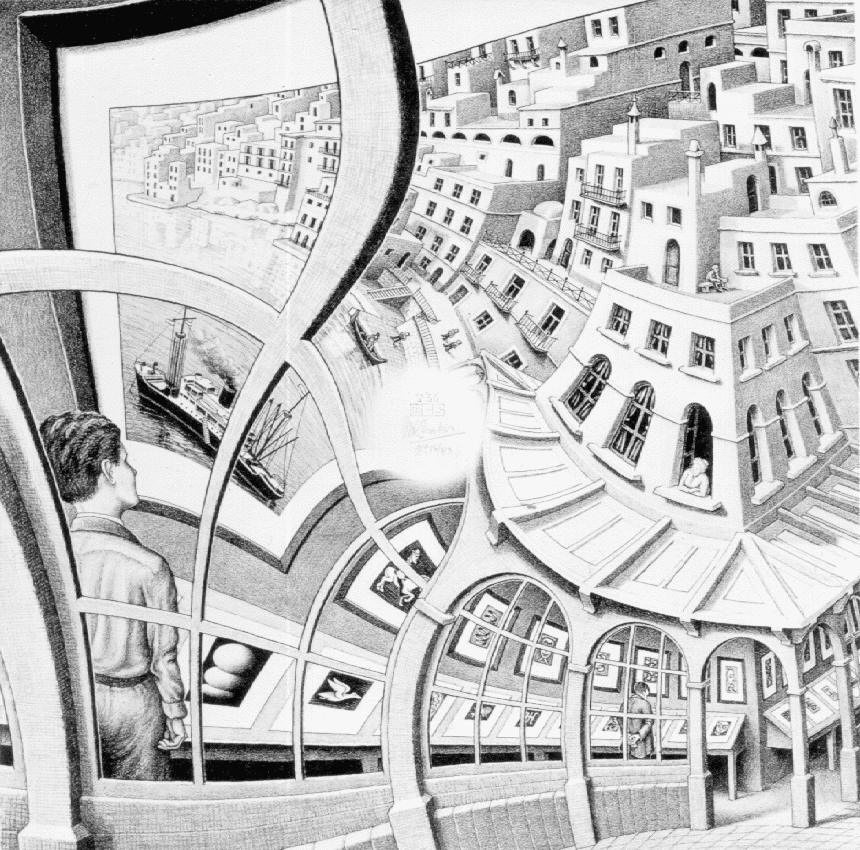
\includegraphics[width=0.5\columnwidth]{GalleriaStampe} 
\caption[Un esempio di figura mobile]{Un esempio di figura mobile (l'immagine, che riproduce la litografia \emph{Galleria di stampe}, di M.~Escher,\index{Escher, M.~C.} proviene da \url{http://www.mcescher.com/}).}
\label{fig:galleria} 
\end{figure}

La figura~\vref{fig:galleria} fornisce un esempio di figura mobile.

\lipsum[3]

\begin{figure}[tb]
\centering
\subfloat[Asia personas duo.]
{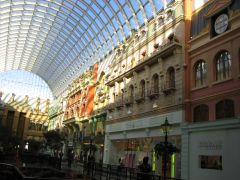
\includegraphics[width=.45\columnwidth]{Lorem}} \quad
\subfloat[Pan ma signo.]
{\label{fig:ipsum}%
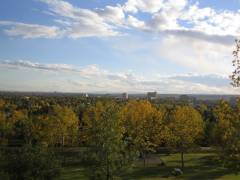
\includegraphics[width=.45\columnwidth]{Ipsum}} \\
\subfloat[Methodicamente o uno.]
{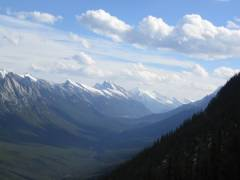
\includegraphics[width=.45\columnwidth]{Dolor}} \quad
\subfloat[Titulo debitas.]
{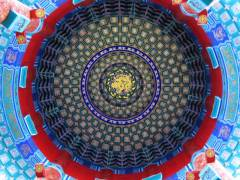
\includegraphics[width=.45\columnwidth]{Sit}}
\caption[Tu duo titulo debitas latente]{Tu duo titulo debitas
latente.}
\label{fig:esempio}
\end{figure}

La figura~\vref{fig:esempio} costituisce un esempio di figura mobile.

\lipsum[4]

% !TEX encoding = UTF-8
% !TEX TS-program = pdflatex
% !TEX root = ../tesi.tex
% !TEX spellcheck = it-IT

%*******************************************************
% Acronimi
%*******************************************************
\cleardoublepage
\manualmark
\phantomsection 
\addcontentsline{toc}{chapter}{\tocEntry{\acroname}}
\chapter*{\acroname\markboth{\spacedlowsmallcaps{\acroname}}{\spacedlowsmallcaps{\acroname}}}
\begin{acronym}[CTBNC] % insert in the square brackets the longest acronym word
    \acro{BN}[BN]{\bn}
    \acro{CIM}[CIM]{\cim}
    \acro{CTBN}[CTBN]{\ctbn}
    \acro{CTBNC}[CTBNC]{\ctbnc}
    \acro{DAG}[DAG]{\ul{Directed acyclic graph}{grafo aciclico diretto}}
    \acro{IM}[IM]{\im}
\end{acronym}

% !TEX encoding = UTF-8
% !TEX TS-program = pdflatex
% !TEX root = ../tesi.tex
% !TEX spellcheck = it-IT

%*******************************************************
% Indice analitico
%*******************************************************
\cleardoublepage
\manualmark
\phantomsection
\markboth{\spacedlowsmallcaps{\indexname}}{\spacedlowsmallcaps{\indexname}}
\addcontentsline{toc}{chapter}{\tocEntry{\indexname}}
\pagestyle{scrheadings}
\printindex

% !TEX encoding = UTF-8
% !TEX TS-program = pdflatex
% !TEX root = ../tesi.tex
% !TEX spellcheck = it-IT

%*******************************************************
% Bibliografia
%*******************************************************
\cleardoublepage
\nocite{*}
\printbibliography
% \input{backmatter/glossario} % indice dei termini
% !TEX encoding = UTF-8
% !TEX TS-program = pdflatex
% !TEX root = ../tesi.tex
% !TEX spellcheck = it-IT

%*******************************************************
% Dichiarazione
%*******************************************************
\cleardoublepage
\phantomsection
\pdfbookmark{Dichiarazione}{Dichiarazione}
\chapter*{Dichiarazione}
\thispagestyle{empty}

Lorem ipsum dolor sit amet, consectetuer adipiscing elit. Ut purus elit, vestibulum ut, placerat ac, adipiscing vitae, felis. Curabitur dictum gravida mauris. Nam arcu libero, nonummy eget, consectetuer id, vulputate a, magna. Donec vehicula augue eu neque.

Pellentesque habitant morbi tristique senectus et netus et malesuada fames ac turpis egestas. Mauris ut leo. Cras viverra metus rhoncus sem. Nulla et lectus vestibulum urna fringilla ultrices.

\bigskip
 
\noindent\textit{\myLocation, \MakeTextLowercase{\myTime}}

\smallskip

\begin{flushright}
    \begin{tabular}{m{5cm}}
        \\ \hline
        \centering\myName \\
    \end{tabular}
\end{flushright}

\end{document}
